\section{Empirical Results}
We begin with numerical results obtained for determining sensing locations by application of kernel observers to the prediction of spatiotemporal functions. The highlight here is a set of results on sensing global ocean temperatures with information from just a few locations using the AVHRR satellite data. This is followed by an application of E-GP in predicting spatiotemporal functions. We include results in predicting weed growth in simulated agricultural fields. The application of E-GP to model flow past a cylinder at different Reynolds numbers is explored in ``\nameref{sb:cfd}''. We conclude the results section with a comparison of eigenvalues and Koopman modes computed from E-GP to those of DMD. 

\subsection{Sensing Locations for Synthetic Data Sets}\label{sec:exp}
The goal of this experiment is to investigate the dependency of the observability of system \eqref{k_measure} on the shaded observation matrix and the lower bound presented in Proposition \ref{prop:2}. The domain is fixed on the interval $\dom = [0,2\pi]$. First, we pick sets of points $\shCent^{(\setind)} = \{c_1,\dots,c_{\ncent_{\setind}}\}, \ c_{\centind}\in\dom$, $\ncent=50$, and construct a dynamics matrix $\dualop = \JorLa \in {\R^{\ncent \times \ncent}}$, with cyclic index $5$.  We pick the RBF kernel $\kernel(x,y) = e^{-\|x-y\|^2/2\s^2}$, $\s=0.02$. Generating samples $\sampSet=\sampSetLong$, $x_{\sampind}\in\dom$ randomly, we compute the $\minmeas$-shaded property and observability for this system. Figure \ref{fig:kobs_small} shows how shadedness is a necessary condition for observability, validating Proposition \ref{prop:1}: the slight gap between shadedness and observability here can be explained due to numerical issues in computing the rank of $\Obs_{\Tset}$. 
 
Next, we  consider a system with a cyclic index $\minmeas=18$ to verify random sensor placement results. We constructed the measurement operator $\empK$ using the heuristic in Remark \ref{rem:1} (Algorithm \ref{alg:samples}), and random sensor selection to generate the sampling locations $\sampSet$. These results are presented in Figure \ref{fig:sample_observability}. The plot for random sampling which has been averaged over $ 100 $ runs, resembles a c.d.f function of an exponential distribution $ F(X=x)=1-\exp(-\lambda x) $. This verifies the claim made in Theorem \ref{thm:r2}, as the probability of becoming unobservable decays exponentially with the number of sensors placed. Also, fitting an exponential distribution, we found that the mean $ \lambda^{-1}$ comes close to the ratio $ {\rands}/{p} $, which is the expected number of randomly placed sensors required for observability as per Theorem \ref{thm:r1}. Note that observability is not achieved if the number of samples $\nsamp < \minmeas$, which is experimental evidence of the result in Proposition \ref{prop:2}. %, although it is more expensive. 
% Finally, using Algorithm \ref{algo:C2}, we estimate the probable sampling locations $\minmeas $ and check whether the system is observable. We repeat Algorithm \ref{algo:C2}, with $N=\minmeas+1$ and so on, until the system is observable. Figures \ref{fig:aa} and \ref{fig:sample_observability} compares two such results of observability phase transition achieved against an approach that randomly selects sampling locations for $M=50$. Both the plots show that with the random approach we need to sample at more locations as compared to our approach in Algorithm \ref{algo:C2}. Also from the figure \ref{fig:aa}, it is clear that even increasing the number of sampling locations does not guarantee observability for random sampling. %Note that we did not compare with information entropy based methods since they are not applicable 
% For each $M$ the experiment was repeated 100 times; table \ref{sample-table} compares the computed average and variance of sampling locations required to achieve observability using sample locations %$ \hat{c}_{sj} $ 
% from Algorithm \ref{algo:C2} and randomly chosen locations. These results further verify the inference made from figures \ref{fig:aa} and \ref{fig:sample_observability}.
 \vspace{-0.1in}
\subsection{Comparison With Nonstationary Kernel Methods on Real-World Data}\label{sec:comparison}
We use three real-world datasets to evaluate and compare the kernel observer with the two different lines of approach for non-stationary kernels  discussed in section on related work. %\ref{sec:related}. 
For the Process Convolution with Local Smoothing Kernel (PCLSK) and Latent Extension of Input Space (LEIS) approaches, we compare with NOSTILL-GP \cite{garg2012AAAI} and \cite{pfingsten2006nonstationary} respectively, on the Intel Berkeley, Irish Wind and Ozone data-sets. 
% Each of these methods were trained on a particular set of data, and the inferred model was used to perform predictions. 

Model inference for the kernel observer involved three steps: 1) picking the Gaussian RBF kernel $\kernel(x,y) = e^{-\|x-y\|^2/2\s^2}$, a search for the ideal $\s$ is performed for a sparse Gaussian Process model (with a fixed basis vector set $\shCent$ selected using the method in \cite{csato2002sparse}. %\footnote
{For the data set discussed in this section, the number of basis vectors were equal to the number of sensing locations in the training set, with the domain for input set defined over $ \R^2 $}; 2) having obtained $\s$, Gaussian process inference is used to generate weight vectors for each time-step in the training set, resulting in the sequence $\weight_\tindex, \tindex\in\{1,\dots,T\}$; 3) matrix least-squares is applied to this sequence to infer $\dualopApprox$ (Algorithm \ref{alg:egp_trans}). For prediction in the autonomous setup, $\dualopApprox$ is used to propagate the state $\weight_{\tindex}$ forward to make predictions with no feedback, and in the observer setup, a Kalman filter (Algorithm \ref{alg:egp_inf}) with $\nsamp$ determined using Proposition \ref{prop:2}, and locations picked randomly, is used to propagate $\weight_{\tindex}$ forward to make predictions. We also compare with a baseline GP (denoted by `original GP'), which is the sparse GP model trained using all of the available data. 

Our first dataset, the Intel Berkeley research lab temperature data, consists of 50 wireless temperature sensors in indoor laboratory region spanning 40.5 meters in length and 31 meters in width ({\url{http://db.csail.mit.edu/labdata/labdata.html}}). Training data consists of temperature data on March 6th 2004 at intervals of 20 minutes (beginning 00:20 hrs) which totals to 72 timesteps. Testing is performed over another 72 timesteps beginning 12:20 hrs of the same day. Out of 50 locations, we uniformly selected 25 locations each for training and testing purposes. Results of the prediction error are shown in box-plot form in Figure \ref{fig:intel_boxplots} and as a time-series in Figure \ref{fig:intel_comp}, note that `Auto' refers to autonomous set up. Here, the cyclic index of $\dualopApprox$ was determined to be $2$, so $\nsamp$ was set to $2$ for the kernel observer with feedback. Note that here, even the autonomous kernel observer outperforms PCLSK and LEIS overall, and the kernel observer with feedback with $\nsamp = 2$ significantly outperforms all other methods, which is why we did not include results with $\nsamp > 2$. 
% \gXX{explain the significance of N=2, cyclic inde etc, why are we not showing the results with increasing number of feedback locations, include discussion or plots of computational performance, this they will surely ask}
%
%Our first dataset is the well known  Intel Berkeley research lab temperature data. It consists of 50 wireless temperature
%sensors in indoor laboratory region spanning 40.5 meters
%in length and 31 meters in width\footnote{\url{http://db.csail.mit.edu/labdata/labdata.html}}. Training data consisted of temperature data from March 6th 2004 at intervals of  20 minutes (beginning 00:20 hrs) which totals to 72 timesteps. Test was performed over another 72 timesteps beginning 12:20 hrs of the same day. Out of 50 locations, we uniformly
%
%selected 25 locations each for training and testing purposes. For observer, we chose $ \nsamp =2 $ based on the inferred $ \dualopApprox $. For a baseline, we separately train a Gaussian process (for each timestep) assuming knowledge of all data, corresponding result is plotted as ``original". Figure \ref{fig:intel_comp} plots the RMS errors in prediction for each time step, these errors are summarized in the form of box-plots in figure \ref{fig:intel_boxplots}. 




The second dataset is the Irish wind dataset, consisting of daily average
wind speed % (in knots = 0.542 m/s) 
data collected from year
1961 to 1978 at 12 meteorological stations in the Republic
of Ireland ({\url{http://lib.stat.cmu.edu/datasets/wind.desc}}). The prediction error  is in box-plot form in Figure \ref{fig:irish_boxplots} and as a time-series in Figure \ref{fig:irish_comp}. Again, the cyclic index of $\dualopApprox$ was determined to be $2$. In this case, the autonomous kernel observer's performance is comparable to PCLSK and LEIS, while the kernel observer with feedback with $\nsamp = 2$ again outperforms all other methods. 

Finally, the Ozone dataset measures ozone concentration (in parts per billion) measured at 60 stations by the United States Environmental Protection Agency \cite{li2006spatiotemporal} across USA. Due to missing measurements, we only selected data from
year 1997 to 2013 for training and evaluation. For each station, we averaged ozone concentration over a period of three months, resulting in four quarters per year.
Out of 60 sensor locations, we uniformly selected 30 for training and the remaining locations for testing purposes. The prediction error results are presented in box-plot form in Figure \ref{fig:ozone_boxplots} and as a time-series in Figure \ref{fig:ozone_comp}. Here, the cyclic index of $\dualopApprox$ was determined to be $1$. In this case, the performance of autonomous kernel observer is comparable to PCLSK and LEIS, with kernel observer with feedback with $\nsamp = 1$ performing the best. Table \ref{tab:timing} reports the total training and prediction times associated with PCLSK, LEIS, and the kernel observer. We observed that, 1) the kernel observer is an order of magnitude faster than the competing methods, and 2) even for small sets, competing methods did not scale well.

%For both datasets, $ \nsamp =2 $ was chosen based on the inferred $ \dualopApprox $ using proposition \ref{prop:2}. In both cases the cyclic index of $ \dualopApprox $ was one. We also investigated prediction errors for chosing sampling locations randomly from the training set. For this we performed 100 runs of experiment, and the results are shown in Table 1. This empirical evidence shows that it suffices to randomly select sampling/sensing locations for Kernel Observer. 
\begin{table}[h]
	\centering
	\caption{Total training and prediction times for Figs. \ref{intel} and \ref{irish} } \label{tab:timing}
		\begin{tabular}{c|ccc}
		\toprule
			{\bf }  & {\bf Intel } & {\bf Irish } &  {\bf Ozone}  \\
			& Berkeley & Wind & \\
			\midrule
			\emph{Data Size}        & 25-72 & 12-36  & {30-68} \\ 
		    (\emph{bases}-\emph{timesteps})                 &       & & \\ \hline
			Kernel Observer         & 2.1 sec & 0.1 sec & 1.61 sec \\
			PCLSK             & 121.4 sec & 7.0 sec & 91.90 sec \\
			LEIS             & 43.8 sec & 2.8 sec & 37.41 sec\\
		\bottomrule
		\end{tabular}
\end{table}
\vspace{-0.1in}
\subsection{Prediction of Global Ocean Surface Temperature}\label{sec:avhhr}
We analyzed the feasibility of our approach on a very large dataset from the National Oceanographic Data Center: the $4$ km AVHRR Pathfinder project, which is a satellite monitoring global ocean surface temperature (Figure \ref{fig:Rawpathfinder} shows the raw data). This dataset is challenging, with measurements at over $37$ million possible coordinates, but with only around 3-4 million measurements available per day, which means a lot of missing data. The goal was to learn the day and night temperature models on data from the year 2011, and then to monitor the system through the year 2012. Success in monitoring would demonstrate two things: 1) the modeling process can capture spatiotemporal trends that generalize across years, and 2) the observer framework allows us to infer the state using a number of measurements that are an order of magnitude fewer than available. Note that due to the size of the dataset and the high computational requirements of the nonstationary kernel methods, a comparison with them was not pursued. To build the autonomous kernel observer and general kernel observer models, we followed the same procedure outlined in Section \ref{sec:comparison}, but with $\shCent=\shCentLong$, $c_{\centind}\in\R^{2}, \ |\shCent| = 300$. The Kalman filter for the general kernel observer model  used $\nsamp \in \{250,500,1000\}$ at random locations to track the system state given a random initial condition $\weight_0$. As a fair baseline, the observers are compared to training a sparse GP model (labeled `original')  on approximately $400,000$ measurements per day. %, to get a fair comparison. 
Figure \ref{fig:pathfinder} is an estimate of global ocean surface temperatures obtained using autonomous kernel observer.
Figures \ref{fig:time_series_day} and \ref{fig:time_series_night} compare the autonomous and feedback approach with $1,000$ samples to the baseline GP; here, it can be seen that the autonomous does well in the beginning, but then incurs an unacceptable amount of error when the time series goes into 2012, i.e. where the model has not seen any training data, whereas FKO does well throughout. 
Figures %13(e)%
\ref{fig:pathfinder_errors_boxplots_day} 
and %13(f) %
\ref{fig:pathfinder_errors_boxplots} 
show a  comparison of the RMS error of estimated values from the real data.
This figure shows the trend of the observer getting better and better state estimates as a function of the number of sensing locations $\nsamp$. Note that we checked the performance of training a GP with only $1,000$ samples as a control, but the average error was about 10 Kelvins, i.e. much worse than FKO.
The time required for using the kernel observer is significantly less than retraining the model every time step; see Figures %13(g)-13(h). 
 \ref{fig:pathfinder_tr_times_boxplots_day}-\ref{fig:pathfinder_tr_times_boxplots_night}.
 
\textbf{Weather Anomaly in 2012:} We further investigated the poor performance of the autonomous kernel observer in the year 2012 as observed in Figures \ref{fig:time_series_day} and \ref{fig:time_series_night}. Clearly, the prediction error blows up at the start of May in the year 2012, indicating that the autonomous model trained using the data from 2011 does well in capturing the annual weather dynamics up to the month of May 2012. We turned our attention towards the weather in May 2012, as changes in ocean temperatures are directly related to the weather. As we guessed, severe weather conditions were reported on the east coast of United States in May 2012, and this anomaly continued over the period of May to June 2012. Here, the apparent poor performance of autonomous kernel observer can actually be a useful indicator in detecting the anomalous behavior, as was the case with the ocean temperature in May 2012 which had deviated from the normal weather dynamics observed in the year 2011 in which no severe weather anomalies were reported. Further, we identified the locations at which the prediction error was two standard deviations above the mean error. These error locations are plotted in Figure \ref{fig:anomaly}. Error locations on 6-7th May coincide with the severe weather onset on the east coast of United states and that of 28-29th May were along the track of storm Beryl approaching the eastern coastline. This shows that the autonomous kernel observer model captures the dynamics of spatiotemporal evolution, and has the potential of identifying current behavior as anomalous to that observed in the training set.
 
\begin{figure}
\centering
    \subfloat[Shaded vs. observability]
    {
    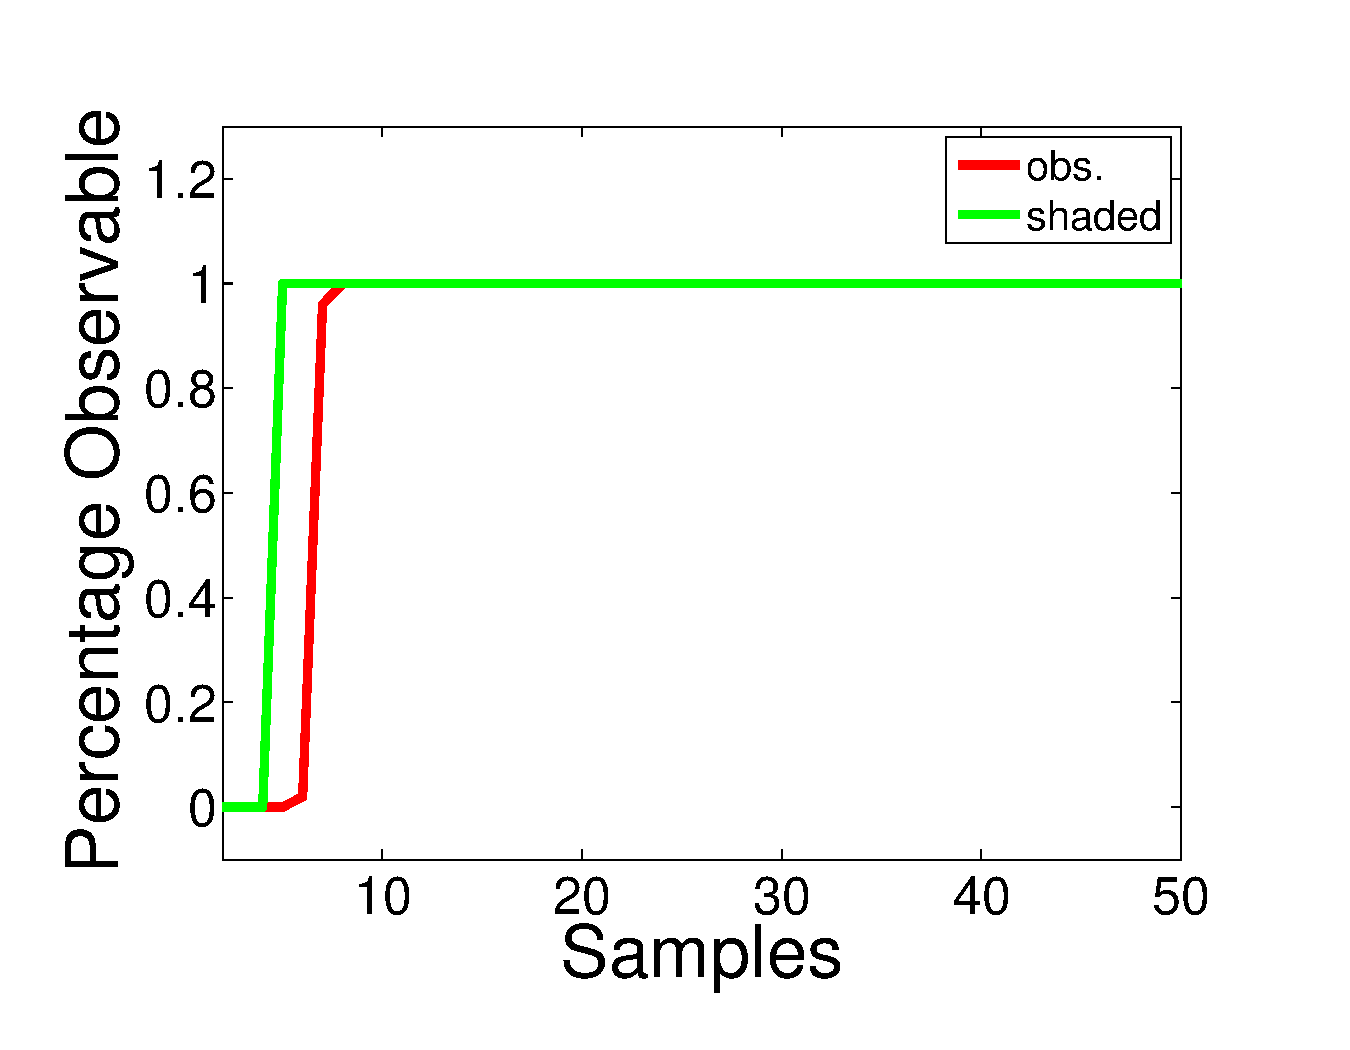
\includegraphics[width=0.45\columnwidth]{kernel_observer_50_cents_smooth4_bandwidth_small.pdf}
    \label{fig:kobs_small}}
     \subfloat[Heuristic vs. random]
     {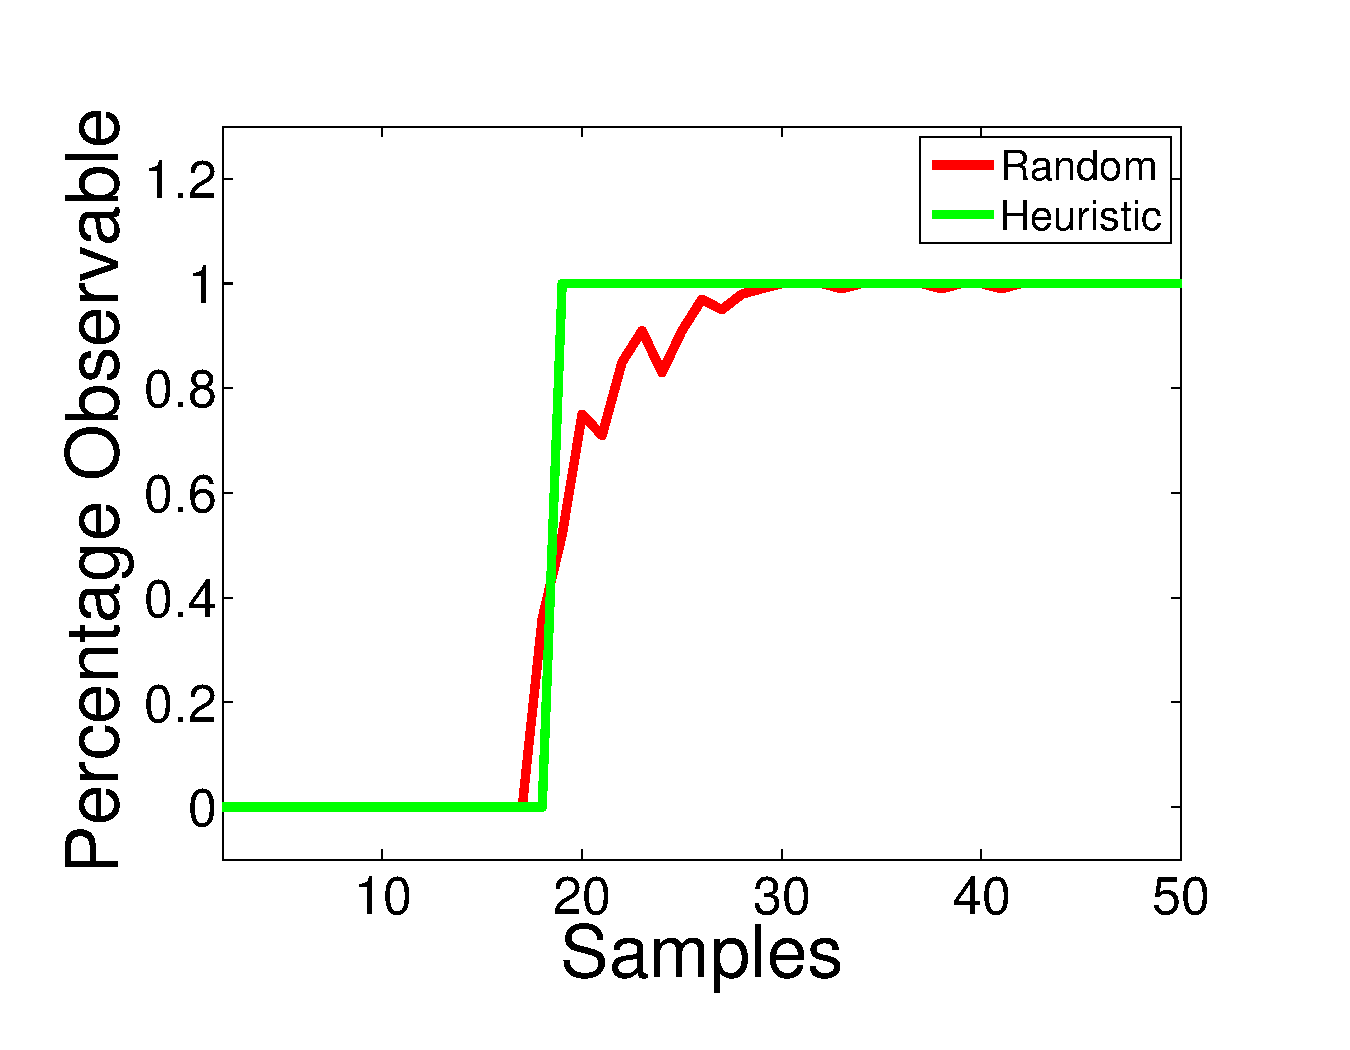
\includegraphics[width=0.45\columnwidth]{rand_average.pdf}
     \label{fig:sample_observability}}  
    \caption{Kernel observability results.}
%\end{figure}
%\begin{figure}[tbh] %{r}{0.5\textwidth}
\end{figure} 

\begin{figure}
\centering
\begin{minipage}{0.8\textwidth}
	% \begin{center}
	\centering
	\subfloat[Error (boxplot)]{
		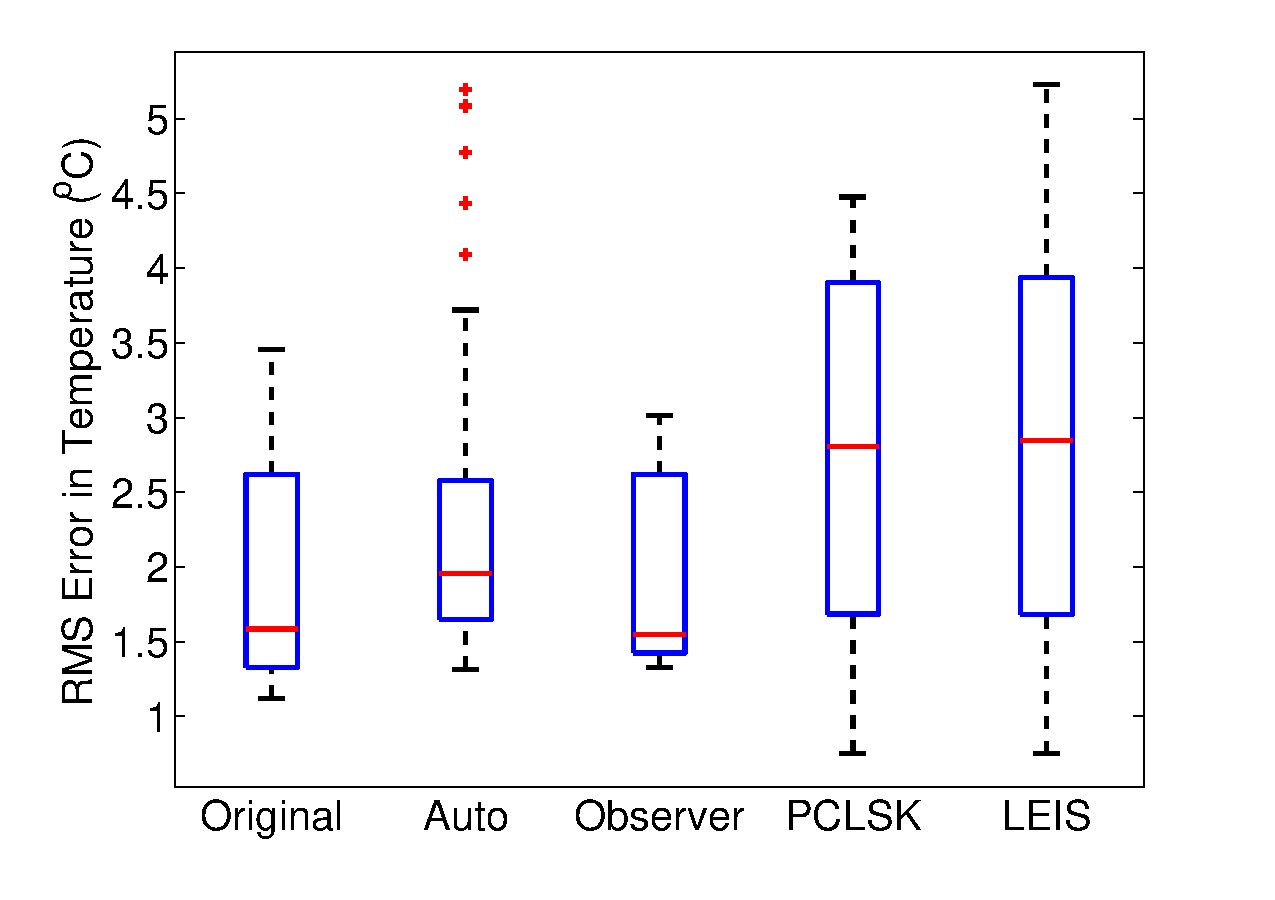
\includegraphics[width=0.48\columnwidth]{box_plot_intel} \label{fig:intel_boxplots} } %pathfinder_errors_boxplot_2012_all_models_night.pdf
	\subfloat[Error (time-series)]
	{
		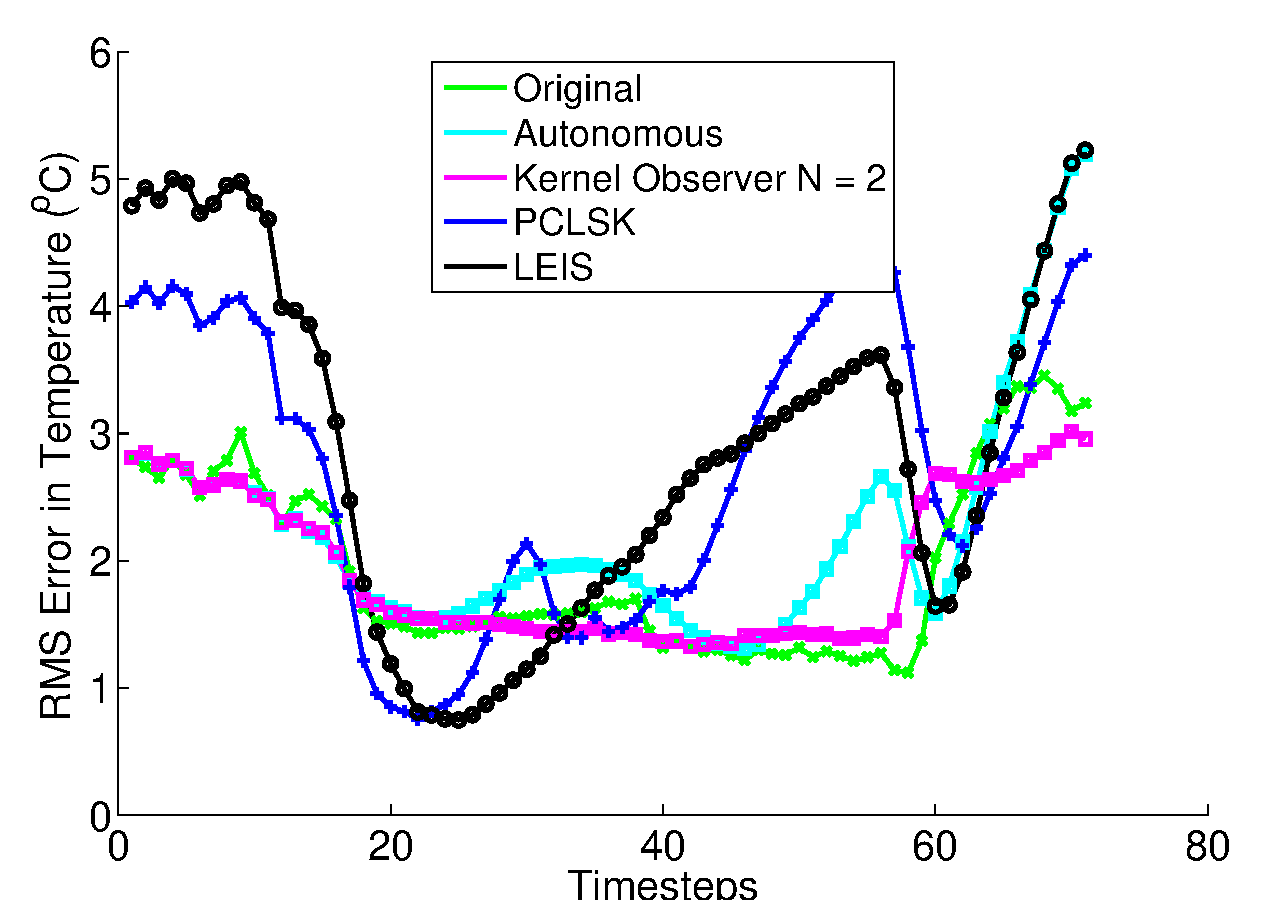
\includegraphics[width=0.48\columnwidth]{Intel_comp} \label{fig:intel_comp}}
	\caption{Comparison of kernel observer to PCLSK and LEIS methods on Intel Berkeley dataset.}     \label{intel}
\end{minipage}\\
\begin{minipage}{0.8\textwidth}
	
		\subfloat[Error (boxplot)]{
		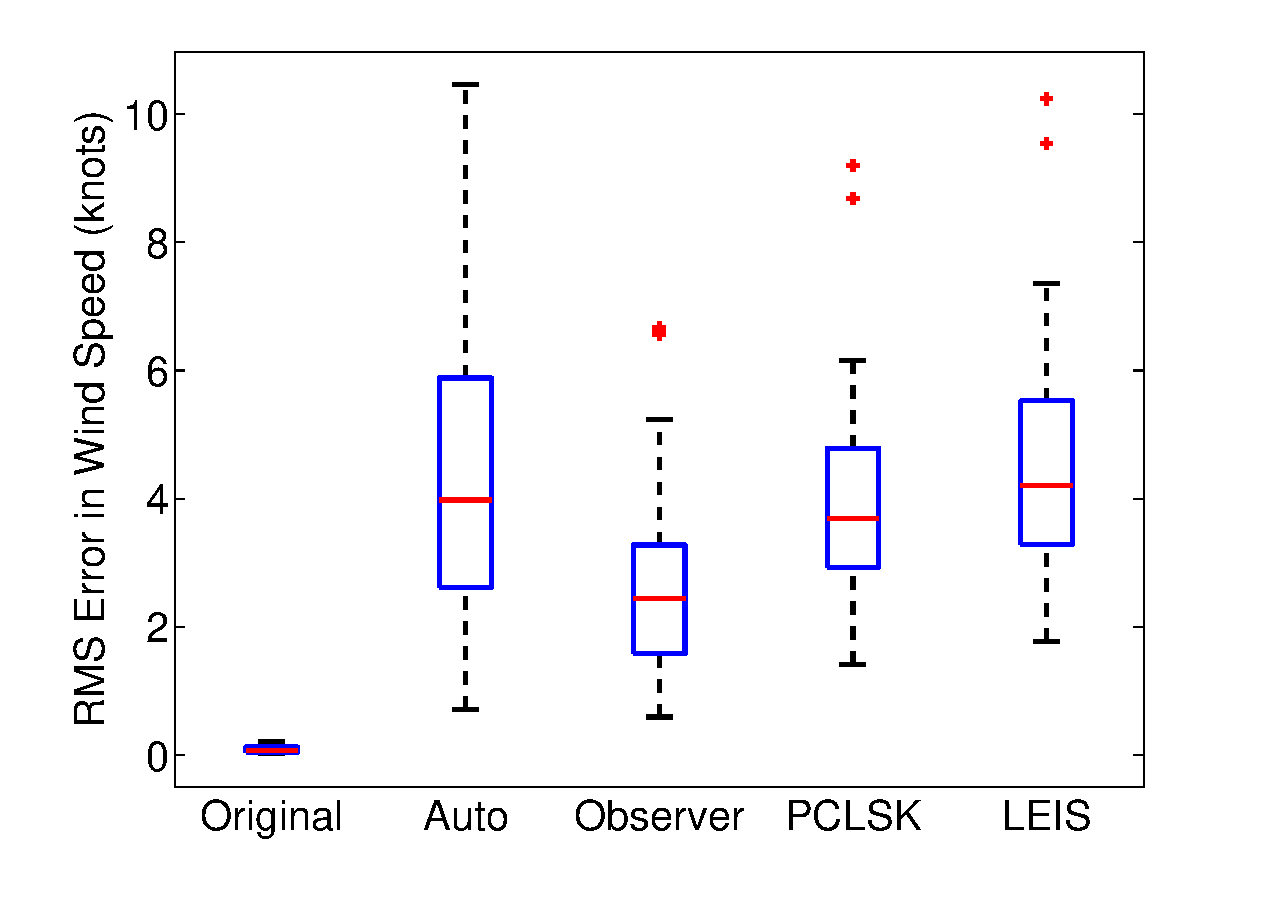
\includegraphics[width=0.48\columnwidth]{box_plot_irish} \label{fig:irish_boxplots} }
		\subfloat[Error (time-series)]{
			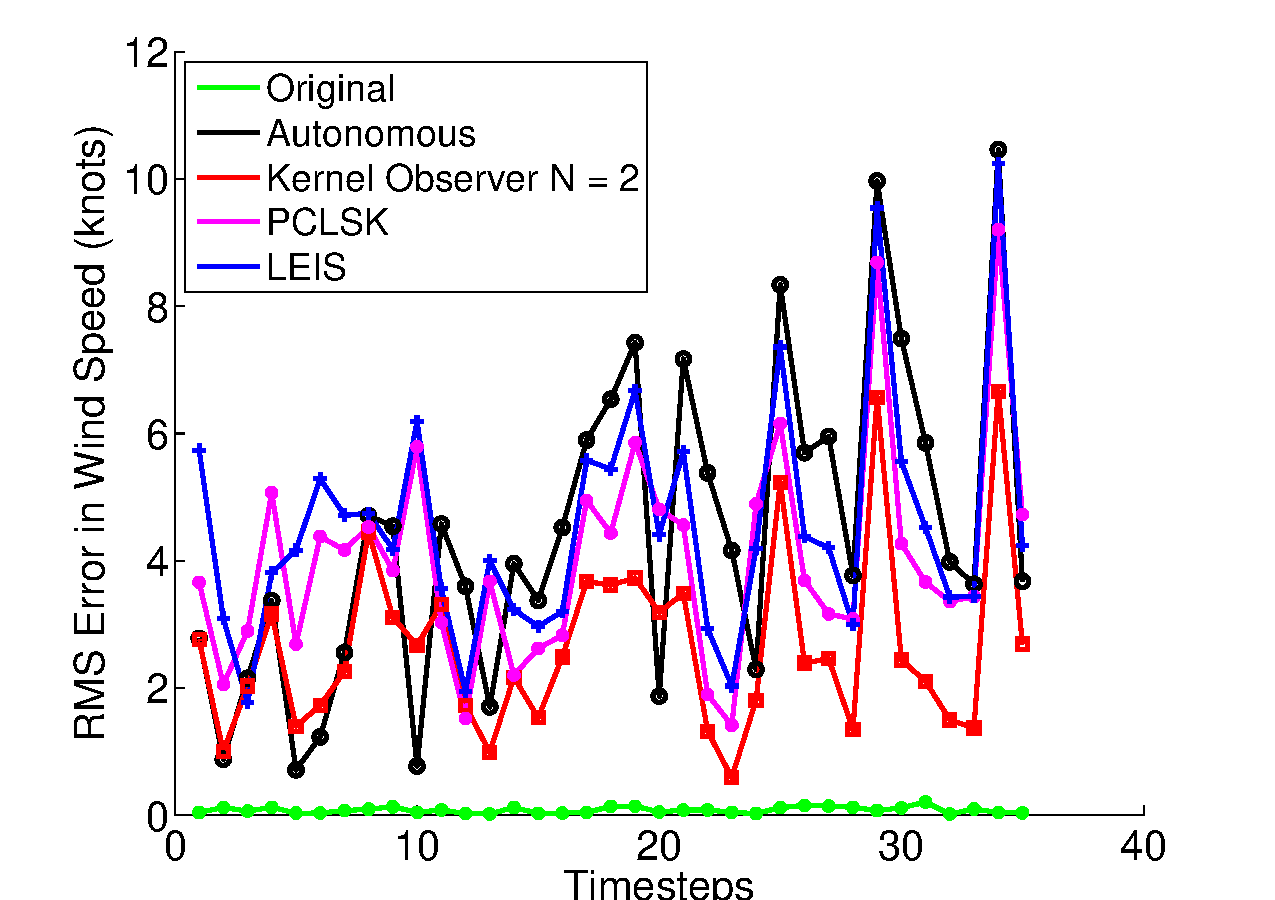
\includegraphics[width=0.48\columnwidth]{irish_wind_comp} \label{fig:irish_comp} }
		\caption{Comparison of kernel observer to PCLSK and LEIS methods on Irish Wind dataset.}\label{irish}
\end{minipage}\\
\begin{minipage}{0.8\textwidth}
	
		\subfloat[Error (boxplot)]{
		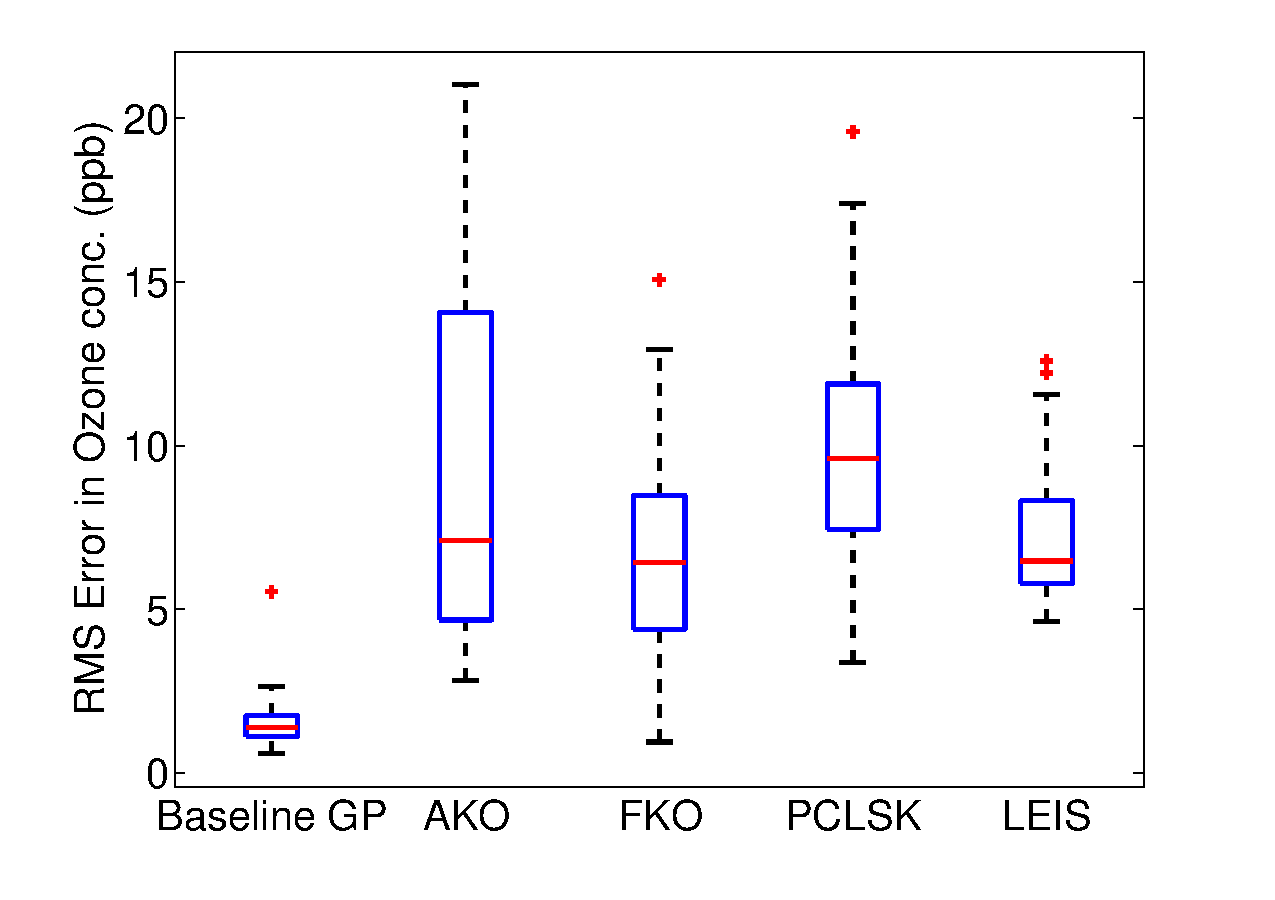
\includegraphics[width=0.48\columnwidth]{box_plot_ozone} \label{fig:ozone_boxplots} }
		\subfloat[Error (time-series)]{
			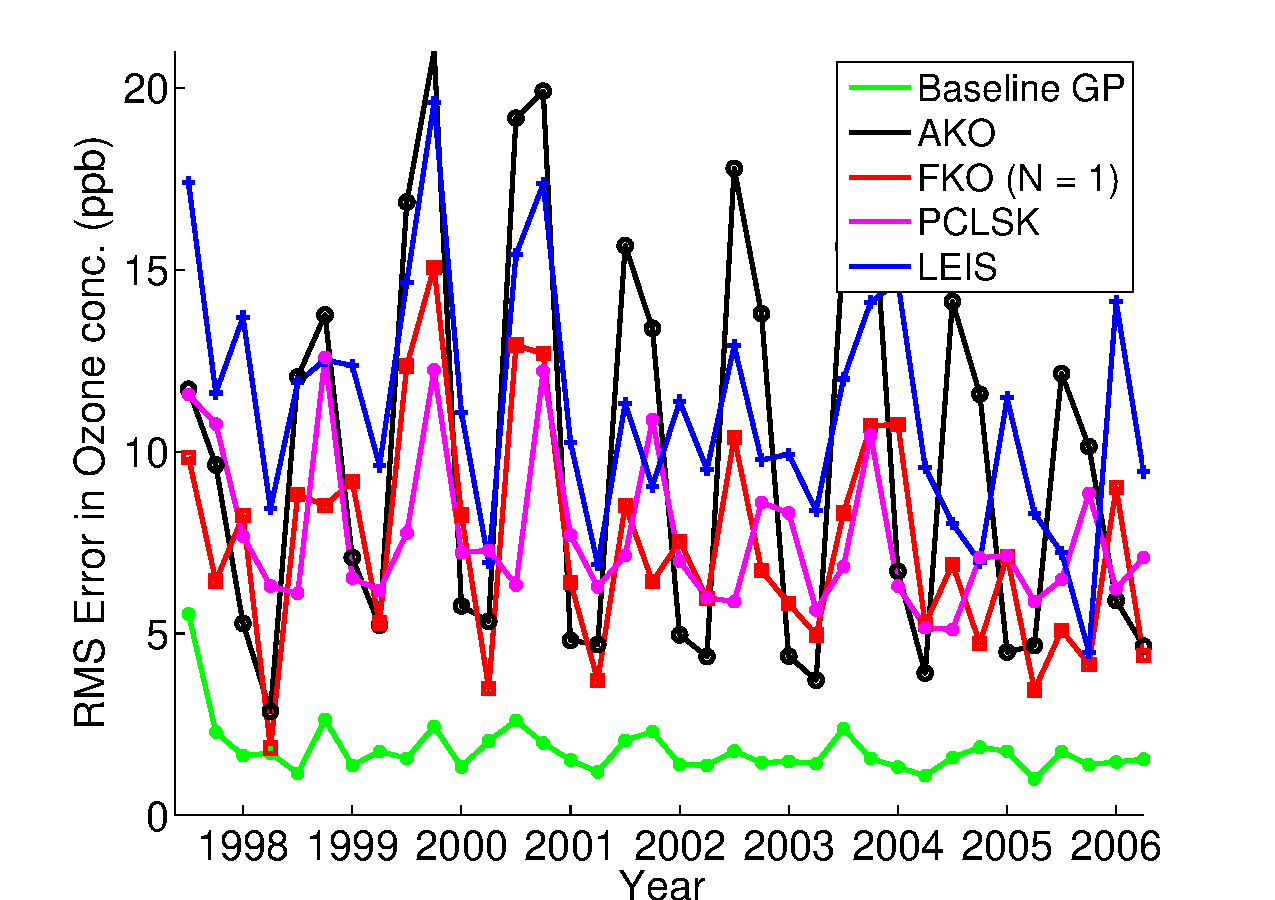
\includegraphics[width=0.48\columnwidth]{ozone_time_series} \label{fig:ozone_comp} }
		\caption{Comparison of kernel observer to PCLSK and LEIS methods on Irish Wind dataset.}\label{ozone}
\end{minipage}
\end{figure}
\begin{figure}
	\centering
	\subfloat[Raw Satellite Data]{
	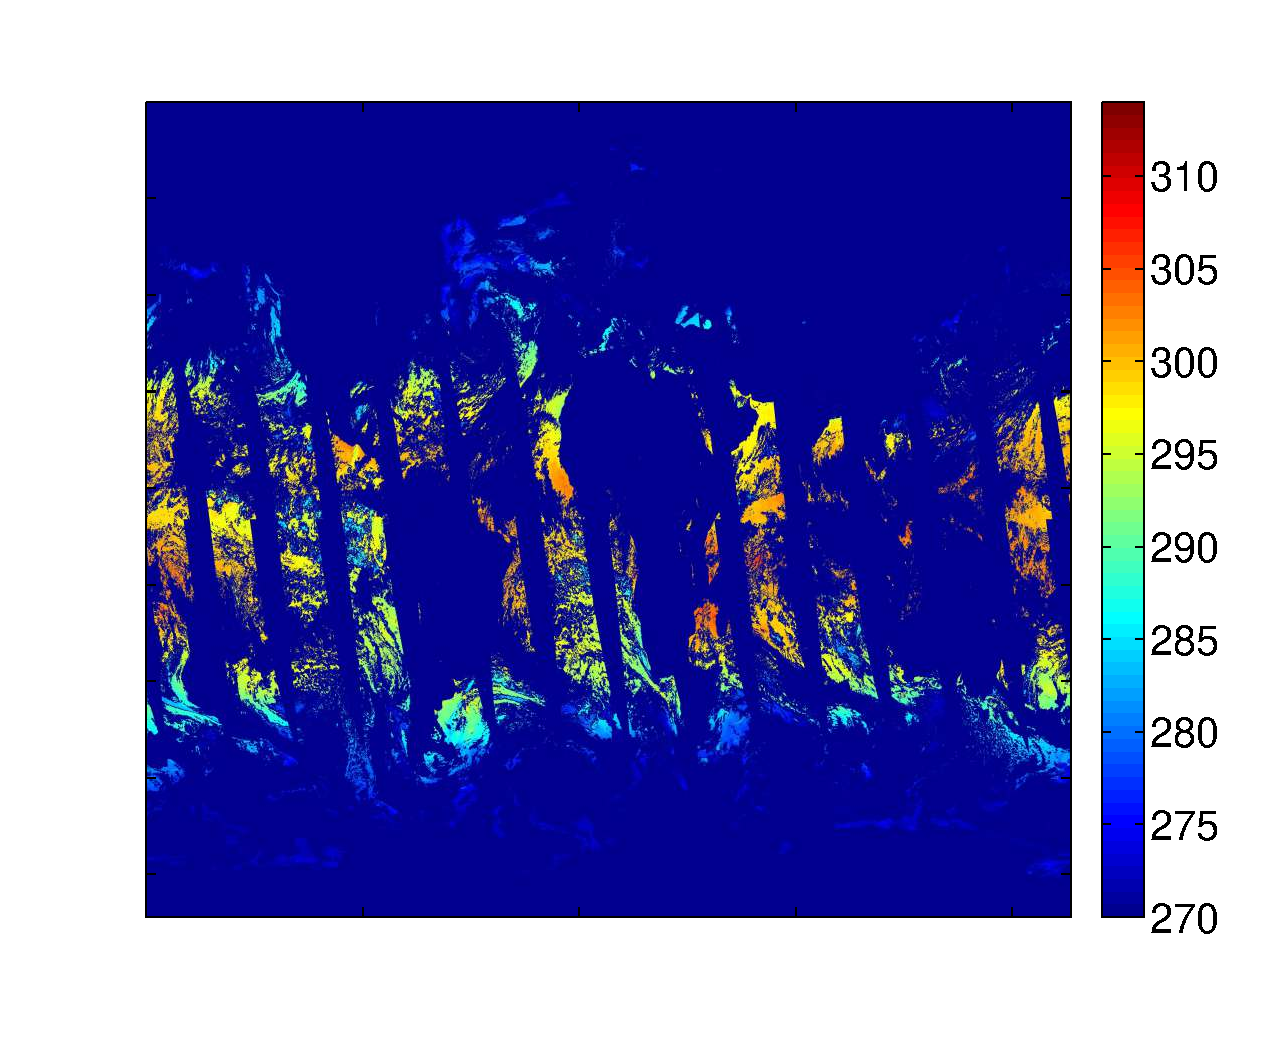
\includegraphics[width=0.4\columnwidth]{pathfinder_raw_data_example}
	\label{fig:Rawpathfinder} }
	\subfloat[AKO estimate]{
	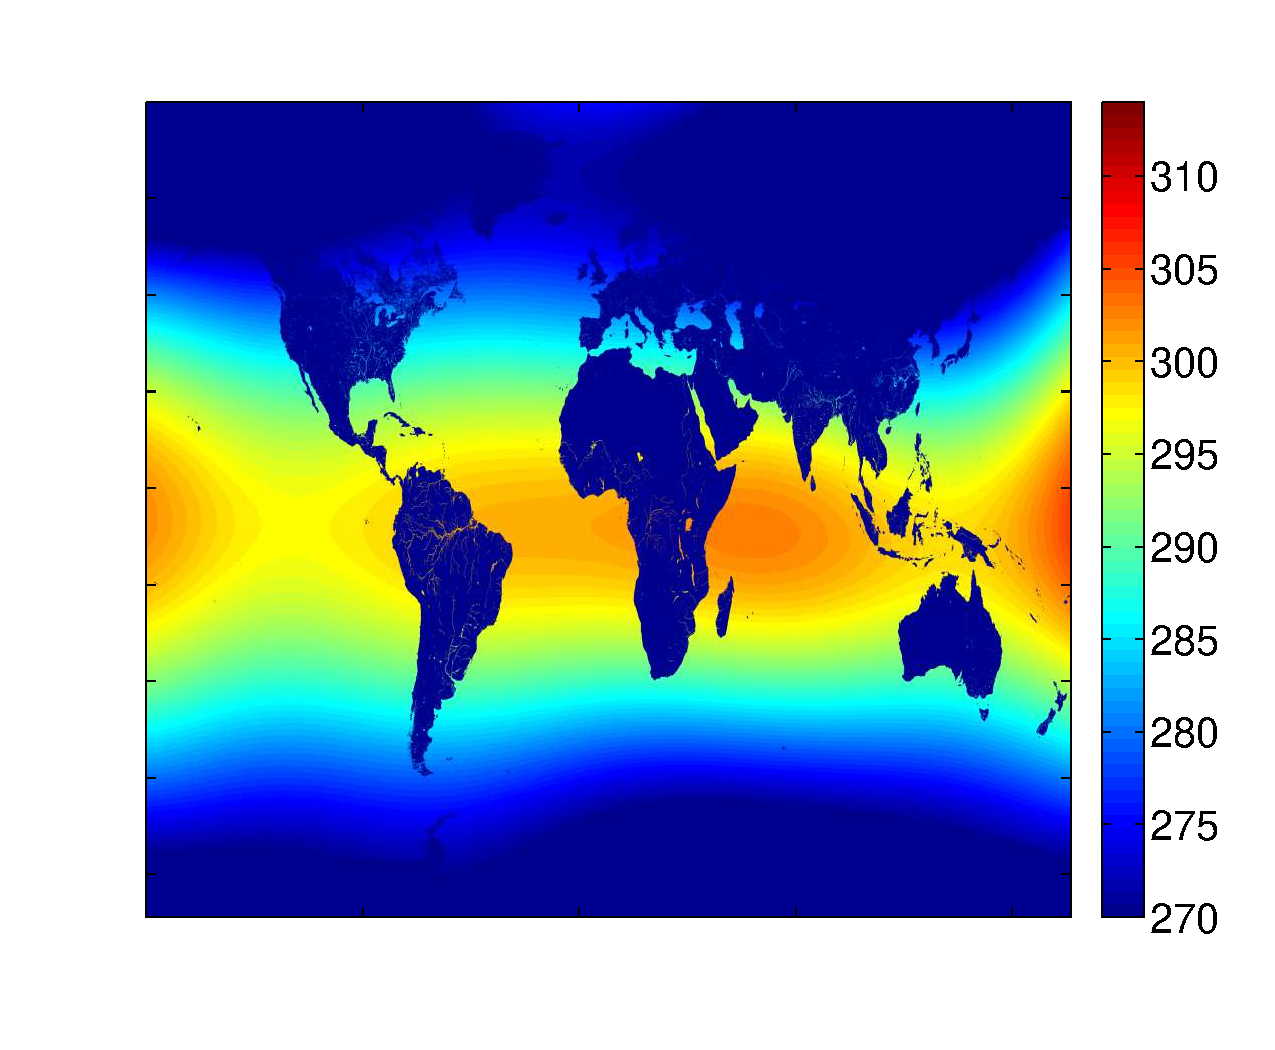
\includegraphics[width=0.4\columnwidth]{pathfinder_inference_example}
	\label{fig:pathfinder} }
	
	\subfloat[Error-day (time-series)]{
		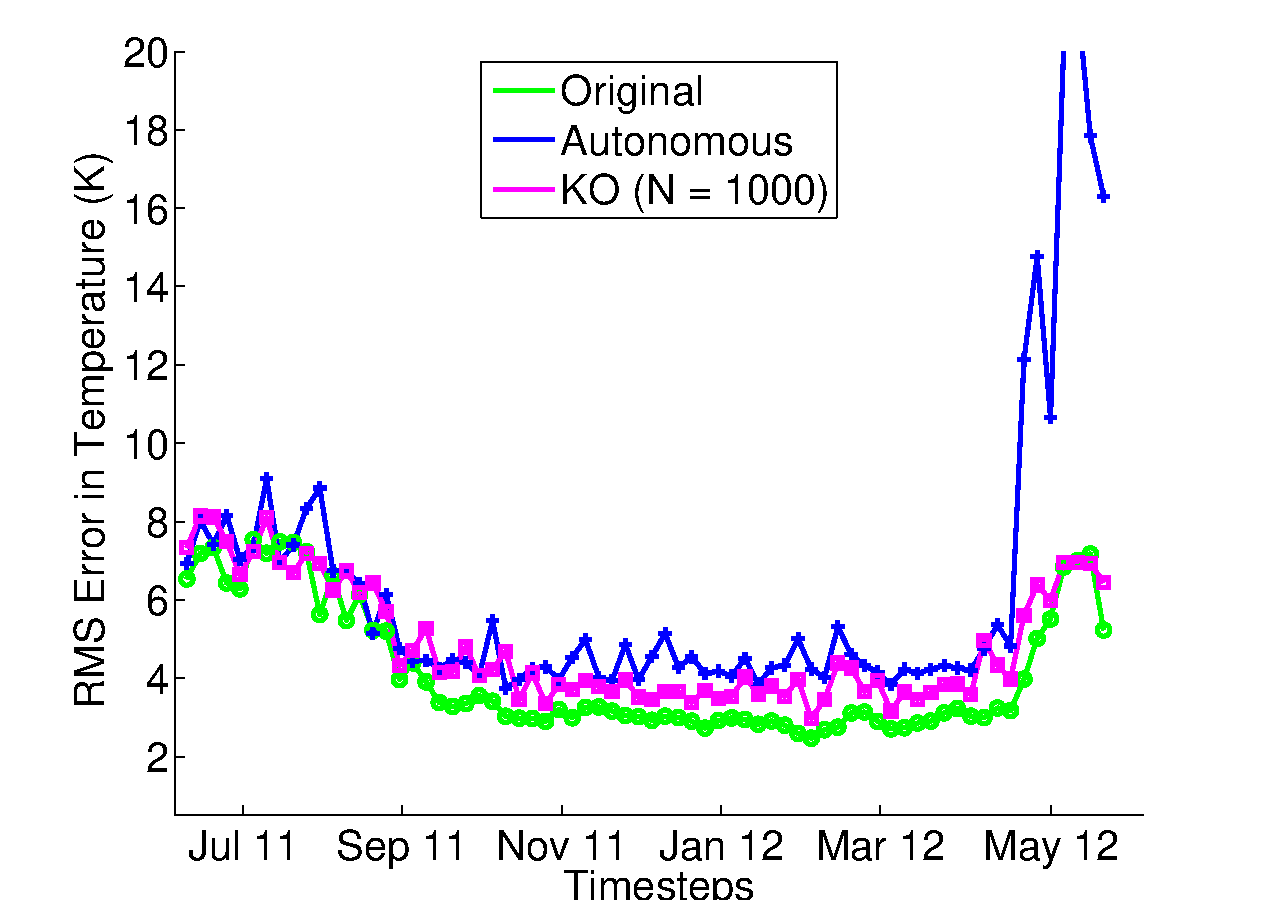
\includegraphics[width=0.4\columnwidth]{time_series_day} \label{fig:time_series_day} }
	\subfloat[Error-night (time-series)]{
		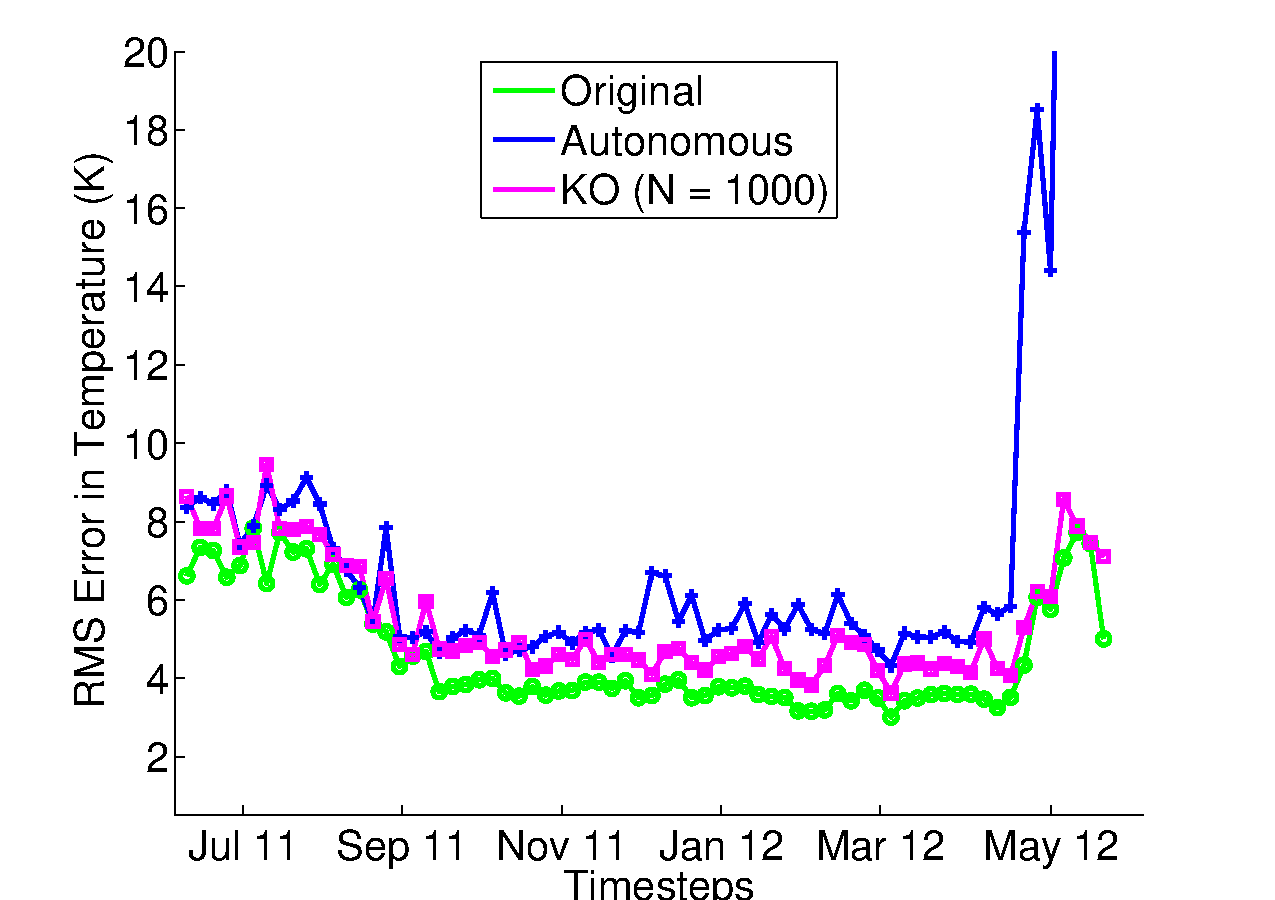
\includegraphics[width=0.4\columnwidth]{time_series_night} \label{fig:time_series_night} }
	 %pathfinder_errors_boxplot_2012_all_models_night.pdf
	 
	\subfloat[Error-day (box-plot)]{
		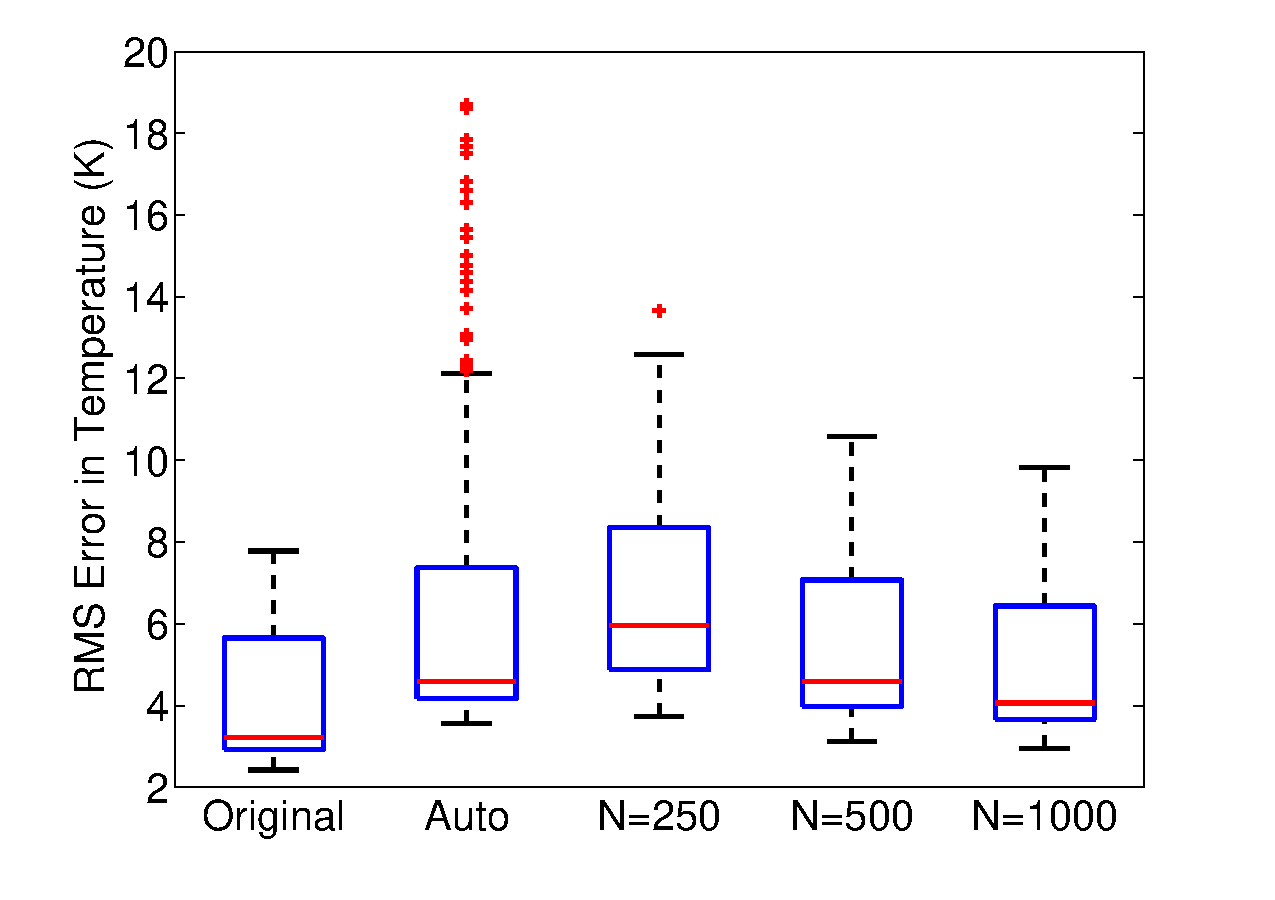
\includegraphics[width=0.4\columnwidth]{box_plot_path_day} \label{fig:pathfinder_errors_boxplots_day} }
	\subfloat[Error-night (box-plot)]{
		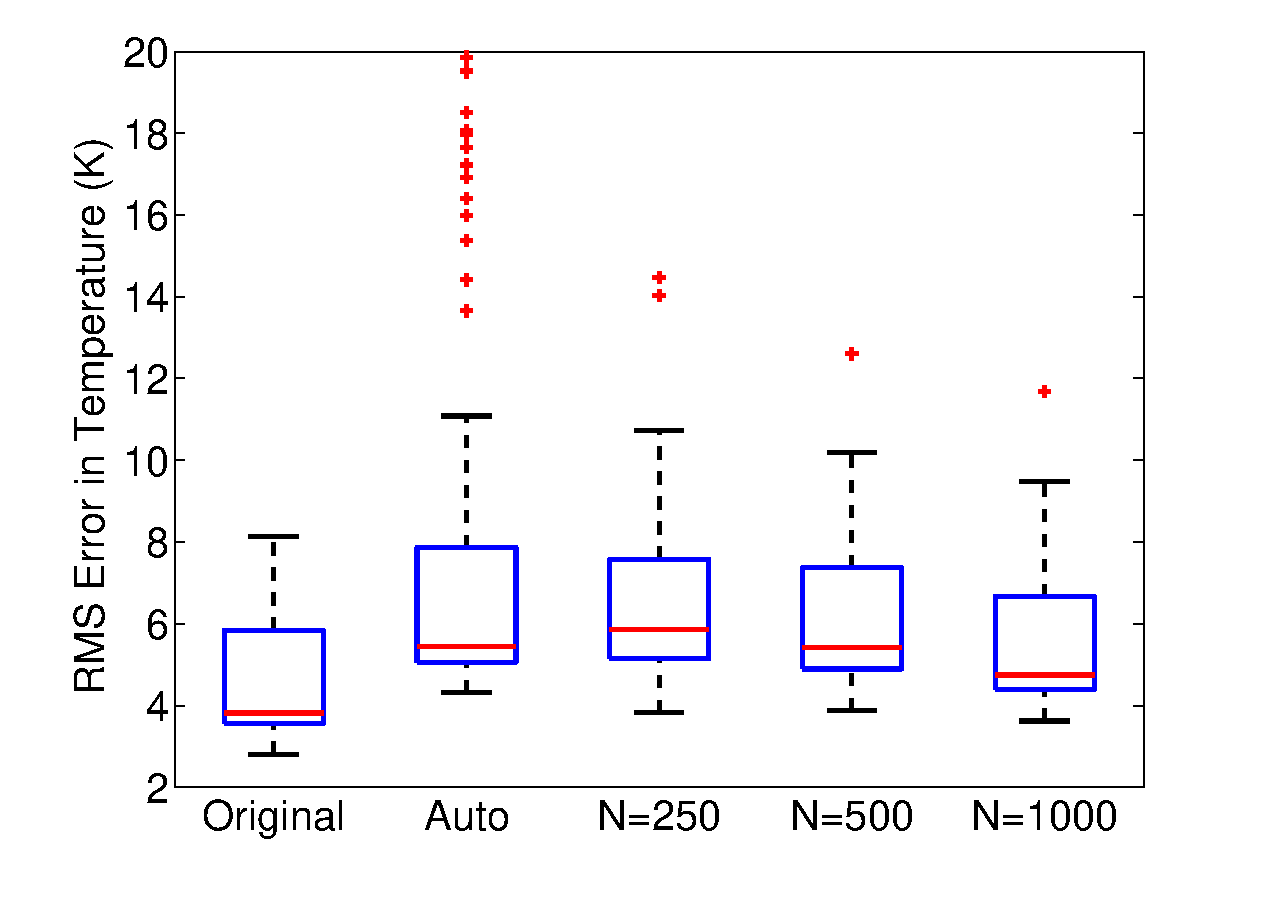
\includegraphics[width=0.4\columnwidth]{box_plot_path} \label{fig:pathfinder_errors_boxplots} }
		
	\subfloat[Estimation time (day)]
	{
		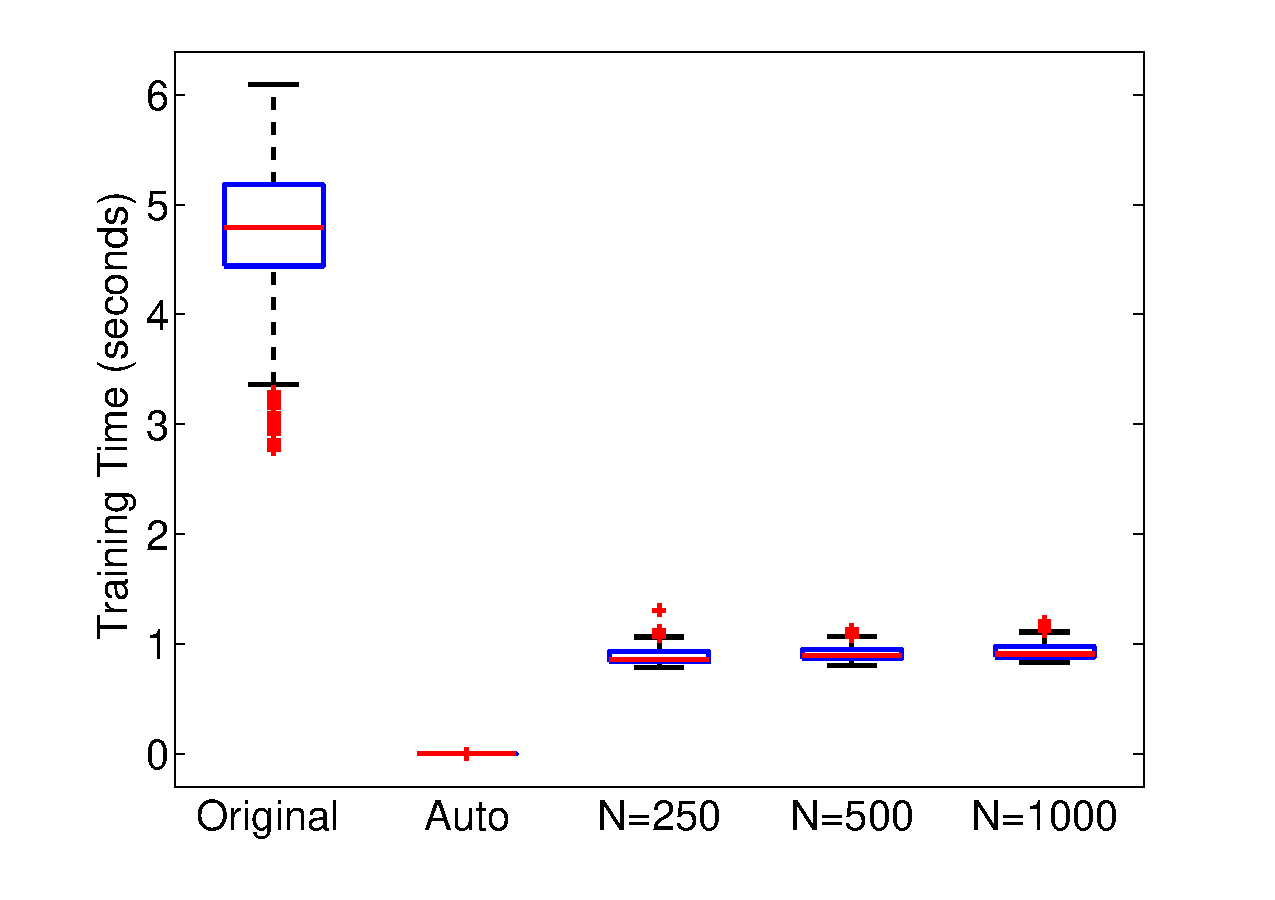
\includegraphics[width=0.4\columnwidth]{box_plot_path_day_time} \label{fig:pathfinder_tr_times_boxplots_day}}
	\subfloat[Estimation time (night)]
	{
		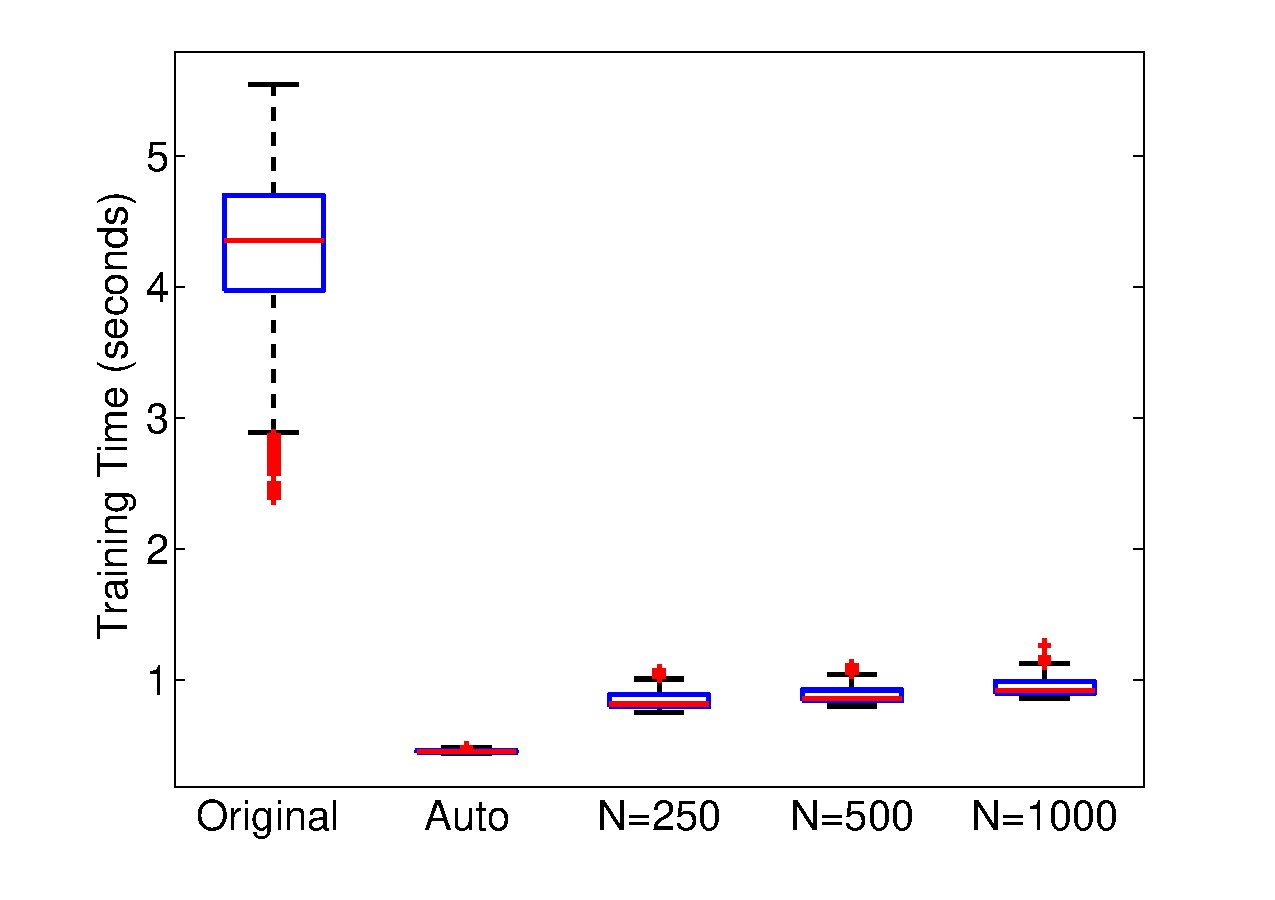
\includegraphics[width=0.4\columnwidth]{box_plot_path_time} \label{fig:pathfinder_tr_times_boxplots_night}}
		
%	\subfloat[Estimation time (night)]
%	{
%		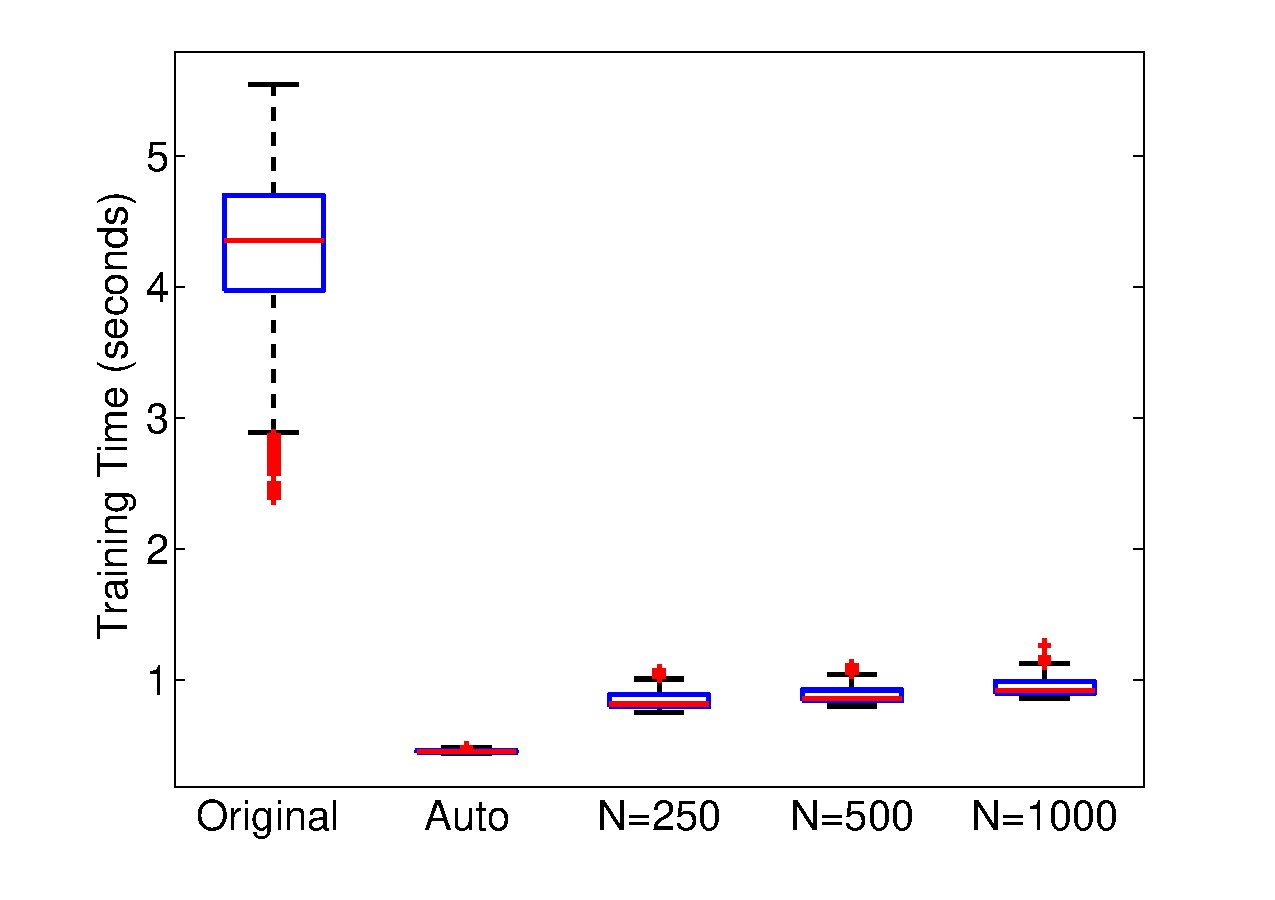
\includegraphics[width=0.33\columnwidth]{box_plot_path_time} \label{fig:pathfinder_tr_times_boxplots}}
	%pathfinder_errors_boxplot_2012_all_models_night.pdf
	%pathfinder_tr_times_boxplot_2012_all_models_night   
	\caption{Performance of the kernel observer over AVVHR satellite 2012 data with different numbers of observation locations.}
\end{figure}

\begin{figure*}
    \centering
    \hspace{-0.3in}\subfloat[6th May]{
	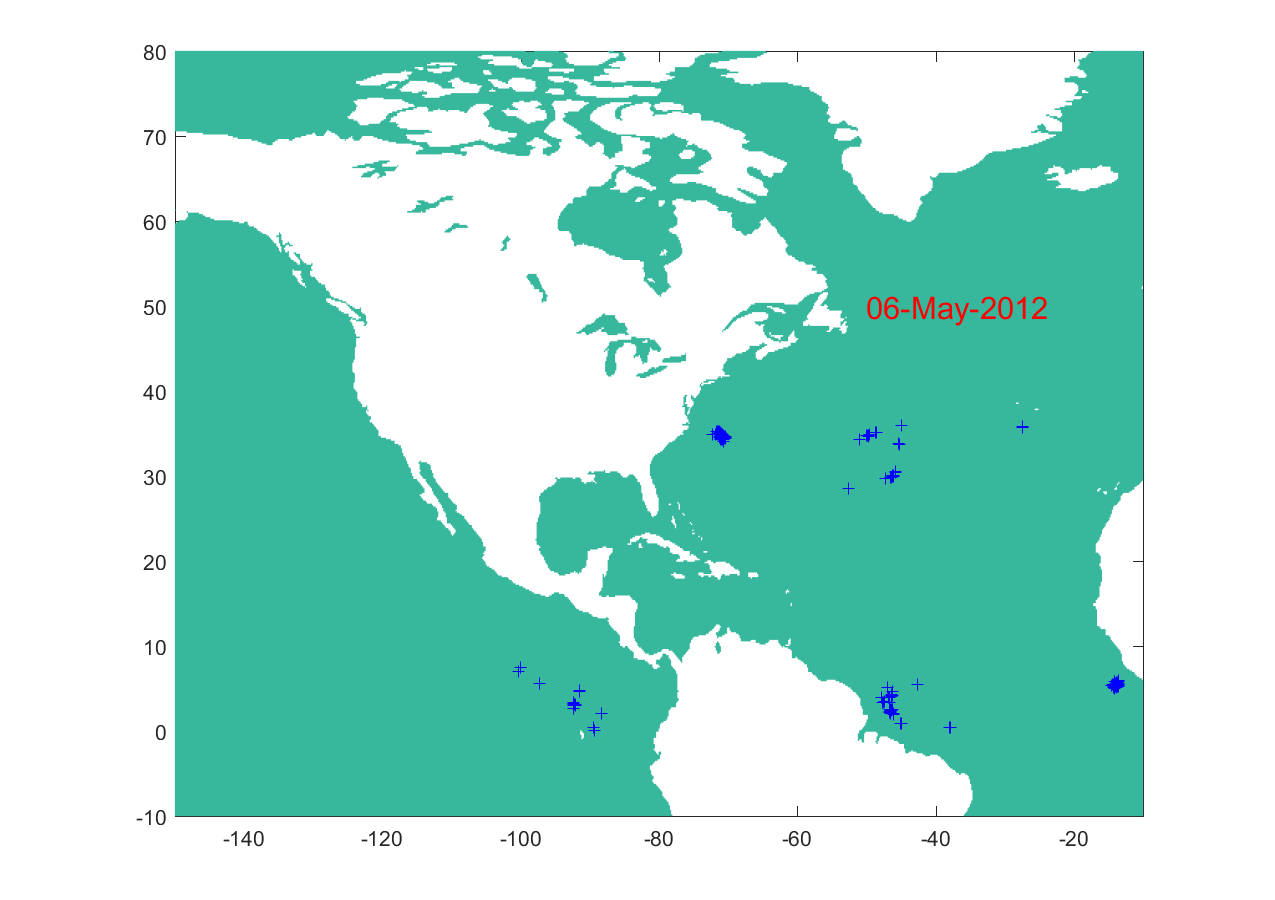
\includegraphics[scale=0.39]{May6}
	\label{fig:May6 } }
	\hspace{-0.5in}
	\subfloat[7th May]{
	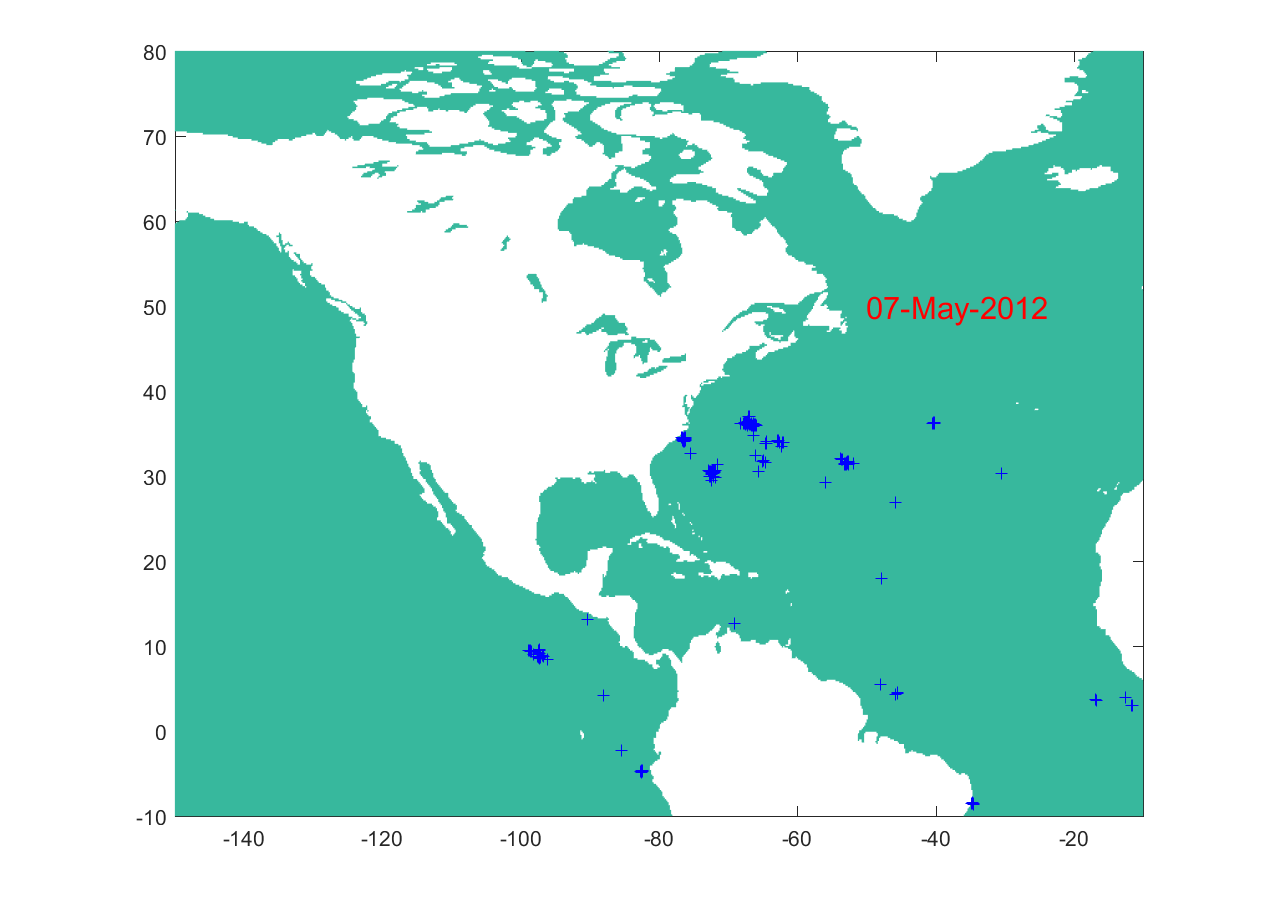
\includegraphics[scale=0.39]{May7}
	\label{fig:May7 } }
	\hspace{-0.5in}
	\subfloat[28th May]{
	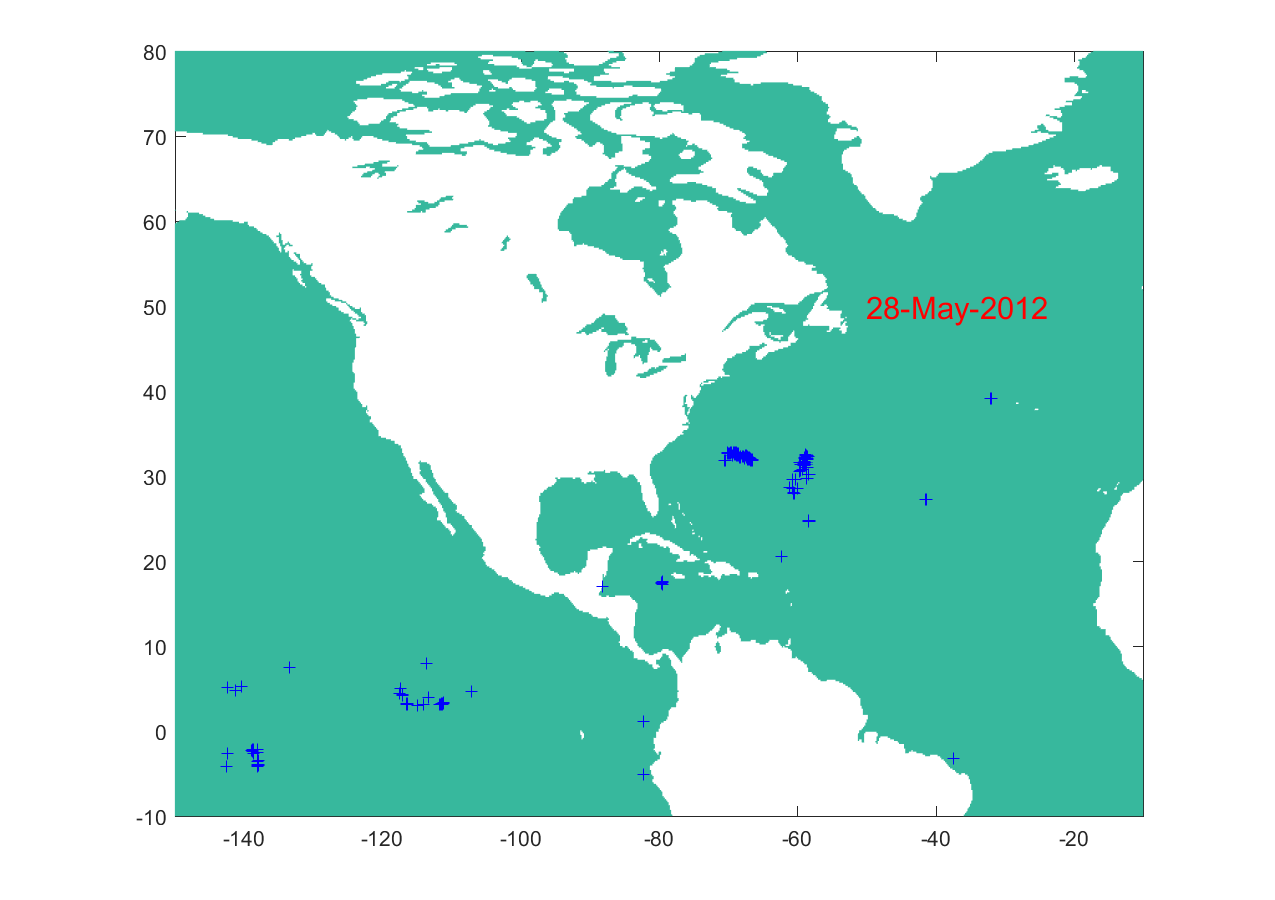
\includegraphics[scale=0.39]{May28}
	\label{fig:May28 } }
	\hspace{-0.5in}\subfloat[29th May]{
	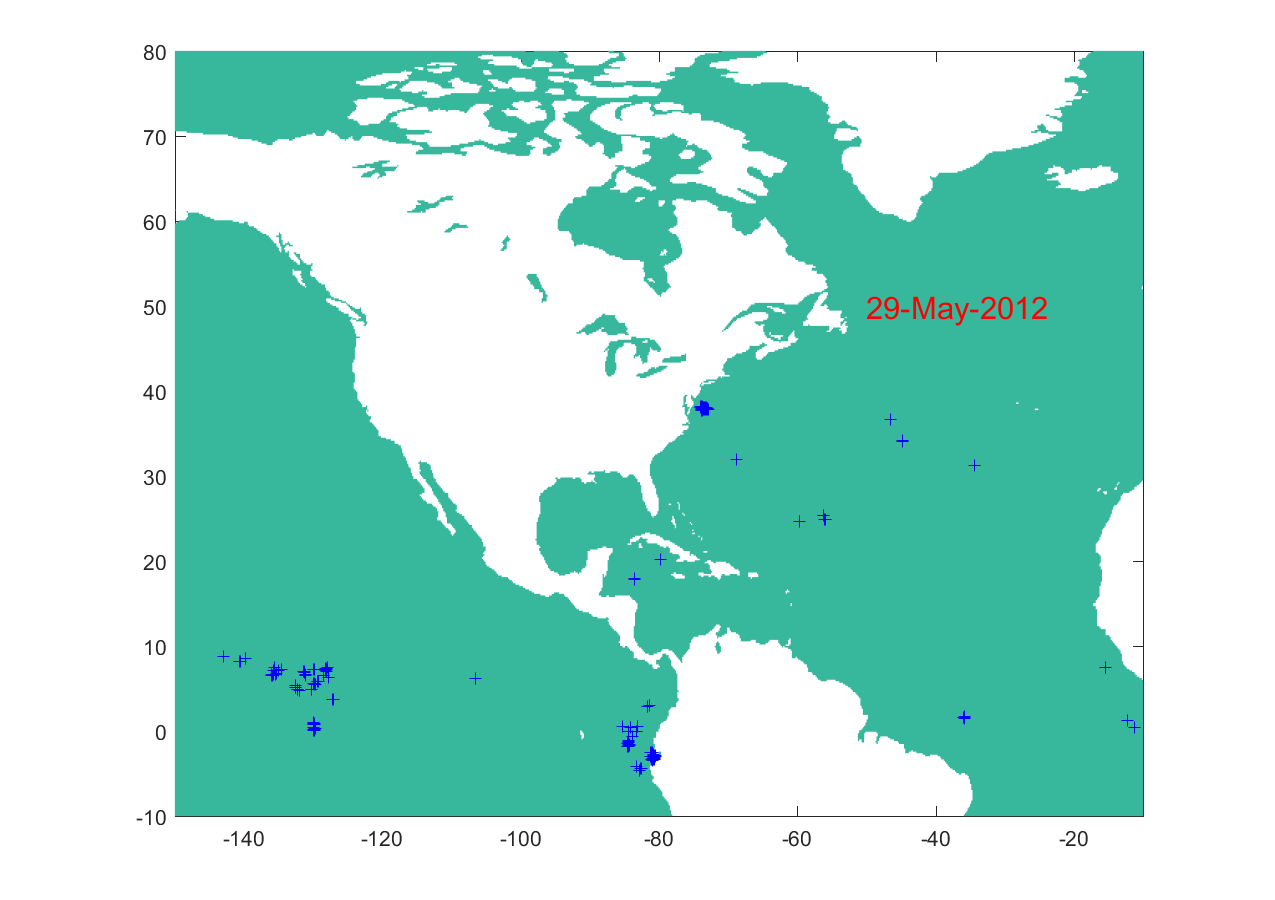
\includegraphics[scale=0.39]{May29}
	\label{fig:May29 } }
	\caption{Locations of weather anomaly obtained based on the error between the acutual temperature and the prediction of autonomous kernel observer. Landmass is shown in white and the ocean is in green. Locations marked have error greater than two standard deviations above the mean error. }
	\label{fig:anomaly}
\end{figure*}



\subsection{Predicting evolution of weed density in agricultural fields}\label{sec:weed}

As a proof-of-concept in applying our methods for learning dynamics and/or inferring the state of spatiotemporally-evolving systems, we examined the problem of predicting weed growth in agricultural fields.

Past work has presented detailed analysis of weed growth models, in which measurements of seed bank density for various species of weeds were conducted \cite{Nordby2018, schutte2014common, sellers2003comparative, horak2000growth}. In order to generate data upon which to test our methods, we implemented a weed growth simulation model whose rate of seedling emergence agrees with that found in the above research \cite{McAllistar18IROS}. A Poisson process is utilized to simulate the temporal evolution of emergence events. This assumption is reasonable over the short time scales in which robots may fully weed a field.
\vskip 1em
Other work in the field of crop science \cite{mulugeta1997seed, mulugeta1999seasonal} has shown that the spatial variation in the seed bank density for some species of weeds may be modeled via the Gini Coefficient of Concentration (GCC). This model is accurate for common waterhemp (\textit{Amaranthus tuberculatus}), and thus we found it useful in our simulation of the spatial distribution of the seed bank density. For more reading. see \cite{davis2013seed, werle2014predicting, McAllistar18IROS} regarding the relationship between seed bank emergence patterns and environmental conditions such as temperature and moisture.

The weed growth simulation is based on Bernoulli random variables, operating on a matrix of cells, each $0.8$ m$^2$, comprising a gridded field of $0.4$ hectares, or a cellular automata model \cite{chopard1998cellular}. Seeds emerge from a limited seed bank, forming a binomial distribution over time. The parameters used, summarized in Table \ref{tab:weedparams}, are aligned with the growth model for common waterhemp determined in \cite{mulugeta1997seed}. The initial density of the seed bank in each cell is $S_0$ on average (between $600$ and $1560$ seeds per cell). However, at the start of the simulation, the seed bank density in each cell, $S_0(x, y)$, is chosen so that Gini Coefficient of Concentration (GCC) between all the cells, used to ensure the relative density of weeds aligns with that seen in real experiments, is from $0.31$ to $0.35$, as was determined experimentally in \cite{mulugeta1997seed}. The field is first divided into fifty patches of weeds, with centers chosen uniformly at random, and sizes from zero to twenty cells in each dimension. Each cell has an initial density between zero and twenty percent of $S_0$, chosen uniformly at random. Finally, for each patch of weeds, up to an additional $S_0$ weeds are added to each cell within each patch, so that the density of each patch follows a normal distribution. 

\begin{table}[h]
	\centering
	\caption{Seed Bank Density Parameters} \label{tab:weedparams} 
	\begin{center}
		\begin{tabular}{ | l | l | l | l | l |}
			\hline
			\textbf{Parameter} & GCC         & $S_0$ (seeds/cell)       & Num. of Patches & Patch Size (Cells in X and Y)  \\ \hline
			\textbf{Range}     & [0.31,0.35] & [600,1560] & 50  & [0,20]  \\ \hline
		\end{tabular}
	\end{center}
\end{table}


Upon initialization of the simulation, a certain number of days, $d_0$, are allowed to elapse before weeding starts. The number of emerging weeds in each cell, $N_{{\text{emerge}}}$, is a randomly generated Poisson variable with mean, $\lambda \left( {x,y,t} \right) $, such that $90$ percent of the seed bank, $S\left( {x,y,t} \right)$, emerges in $T_\text{total}$, which is two months. This emergence rate is aligned with past work \cite{Nordby2018,schutte2014common, werle2014predicting, sellers2003comparative, horak2000growth},  which all present measurements of the seed bank densities for various species of weeds, and provide an analysis of weed growth models for these species.

The weed density in each cell, $\zeta \left( {x,y,t} \right) $, grows as seeds emerge from the seed bank. The maximum weed height at each cell, $\delta \left( {x,y,t} \right)$, increases from zero height at a fixed rate $\Gamma$ inches per day.

The main challenge with weeding robots is that they only have access to sparse data about weed density and height, and no data about the seedbank. In fact, the robots can only sense the row that they are in and potentially the adjacent rows on either side. They have no information about the field in locations that have not been visited. Hence, the robots have to try and predict the global weed density given sparse information. This is a great application for the Kernel observer techniques studied in this paper. To demonstrate the proof of concept, we trained a kernel observer model on the weed density data generated by our simulations, so that robots in the field can quickly infer the state of the field globally from partial measurements from a few rows.

We used Radial Basis Function (RBF) kernels with a bandwidth approximately 5 cells (4.5 meters) wide. These were centered throughout the domain using the algorithm in \cite{csato2001sparse}. After training a GP on each snapshot of the data, we obtained a weight vector trajectory. We used linear least squares do determine the best linear transition in the weight space for this trajectory. Below we have included images of system as predicted by feeding forward the initial condition through this linear transition, as a comparison with the original data. The model is able to approximate the weed density growth data very well, with percent error averaging 5\%. These results show the feasibility of modeling weed growth using E-GPs. Ongoing work involves a massive field campaign to collect the weed density data required to learn these models. Such datasets are currently not available, and the TerraSentia robots discussed in Sidebar: Key control problems in agriculture are being used to collect this data.

\begin{figure*}[h] %{r}{0.5\textwidth}
	\centering
	\subfloat[Snapshot 2]{
		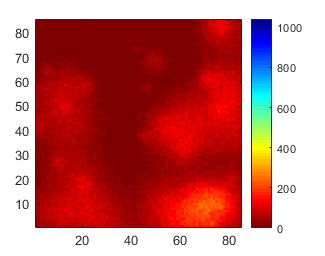
\includegraphics[width=0.23\textwidth]{weed2}		}
	\subfloat[Snapshot 28]{
		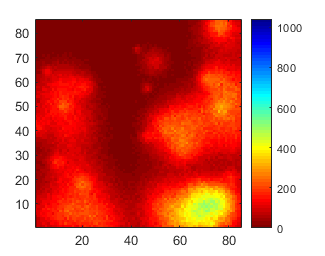
\includegraphics[width=0.23\textwidth]{weed28}		}
	\subfloat[Snapshot 54]{
		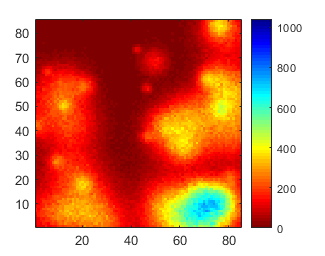
\includegraphics[width=0.23\textwidth]{weed54}		}
	\subfloat[Snapshot 80]{
		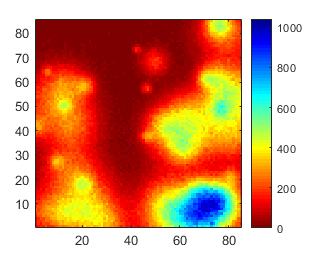
\includegraphics[width=0.23\textwidth]{weed80}		}\\
	\subfloat[Snapshot 2]{
		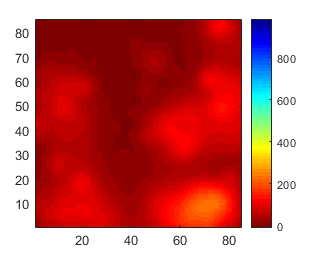
\includegraphics[width=0.23\textwidth]{weed2_egp}		}
	\subfloat[Snapshot 28]{
		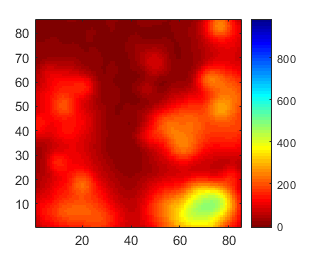
\includegraphics[width=0.23\textwidth]{weed28_egp}		}
	\subfloat[Snapshot 54]{
		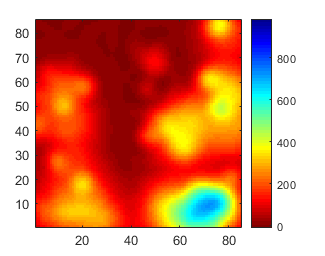
\includegraphics[width=0.23\textwidth]{weed54_egp}		}
	\subfloat[Snapshot 80]{
		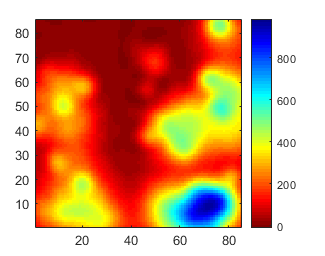
\includegraphics[width=0.23\textwidth]{weed80_egp}		}
	
	\caption{Visualization of Weed Density Growth over 20 days, original (a-d), E-GP (e-h)}
	\label{fig:weed_egp}
\end{figure*}



% \subsection{Control of a linear PDE} %with AVHRR Satellite data}
% We then employed kernel controllers for controlling an approximation to the scalar diffusion equation $u_t = bu_{xx}$ on the domain $\dom=[0,1]$, with $b=0.25$. The solution to this equation is infinite-dimensional, so we chose a kernel $\kernel(x,y) = e^{-(\|x-y\|^2/2\s^2)}$, and a set of atoms  $\Atoms=\shCentLong$, $c_i\in\dom$, with $\ncent = 25$ generating $\fspaceC$, the space approximating $\fspace$, and another set of atoms $\AtomsControl=\{\fmap(d_1),\dots,\fmap(d_{\ncontrol})\}$, $d_j\in\dom$,
% $\ncontrol=13$, generating the control space $\fspaceD$. The number of, and the location of the observations was chosen to be the same as that of the actuation locations $d_j$. First, tests (not reported here) were conducted to ensure that the solution to the diffusion equation is well approximated in $\fspaceC$. Matrix least-squares was used to infer $\estsysop$. Figure \ref{fig:uncontrolled_pde} shows an example of an initial function $f_{\text{init}}$ evolving according to the PDE.  A reference function $f_{\text{ref}}\in\fspaceC$ was chosen to drive $f_{\text{init}}$ to $f_{\text{ref}}$ under the action of the PDE. Finally, Algorithm \ref{alg:egp_control} was used to control the PDE, driving $f_{\text{init}}$ to $f_{\text{ref}}$; Figure \ref{fig:controlled_pde_error} shows the absolute value of the error between $f_k $ and $f_{\text{ref}}$ as a function of time. 

% We performed experiments to evaluate the number of randomly placed Actuators and Sensors required as compared to the lower bound obtained in Proposition \ref{prop:2}. Results in Table \ref{compare} shows that randomly placing the sensors and actuators works efficiently for lower set of atoms $ \ncent$ in $ \Atoms$.
% 
% \begin{table}
% 	\caption{Number of randomly placed Actuators and Sensors (average $\pm$ variance) required as compared to the lower bound $\minmeas$ obtained in Proposition \ref{prop:2}. }
% 	\label{compare}
% 	\begin{center}
% 		\begin{tabular}{|c||c||c||c|}
% 			\hline
% 			Set of & Lower  & Number of   & Number of  \\
% 			Atoms & bound ($\minmeas$) & Actuators  &  Sensors \\
% 			
% 			\hline
% 			M = 25 & 10 & 10.27 $\pm$ 0.45 & 10.36 $\pm$ 0.50 \\
% 			M = 30 & 13  & 15.26 $\pm$ 0.51 & 15.24 $\pm$ 0.49 \\
% 			M = 35 & 19  & 21.43 $\pm$ 0.54 & 21.35 $\pm$ 0.50 \\
% 			M = 40 & 24 & 33.08 $\pm$ 6.05 & 32.40 $\pm$ 6.0 \\
% 			% M = 30 & 8.5 $\pm$ 0.8 & 8.5 $\pm$ 0.9 & 10.8 $\pm$ 1.4 \\
% 			\hline
% 		\end{tabular}
% 	\end{center}
% \end{table}

% \begin{figure}[tbh] %{r}{0.5\textwidth}
%     \centering
%     \subfloat[Evolution of initial function $f_{\text{init}}$.]{
%     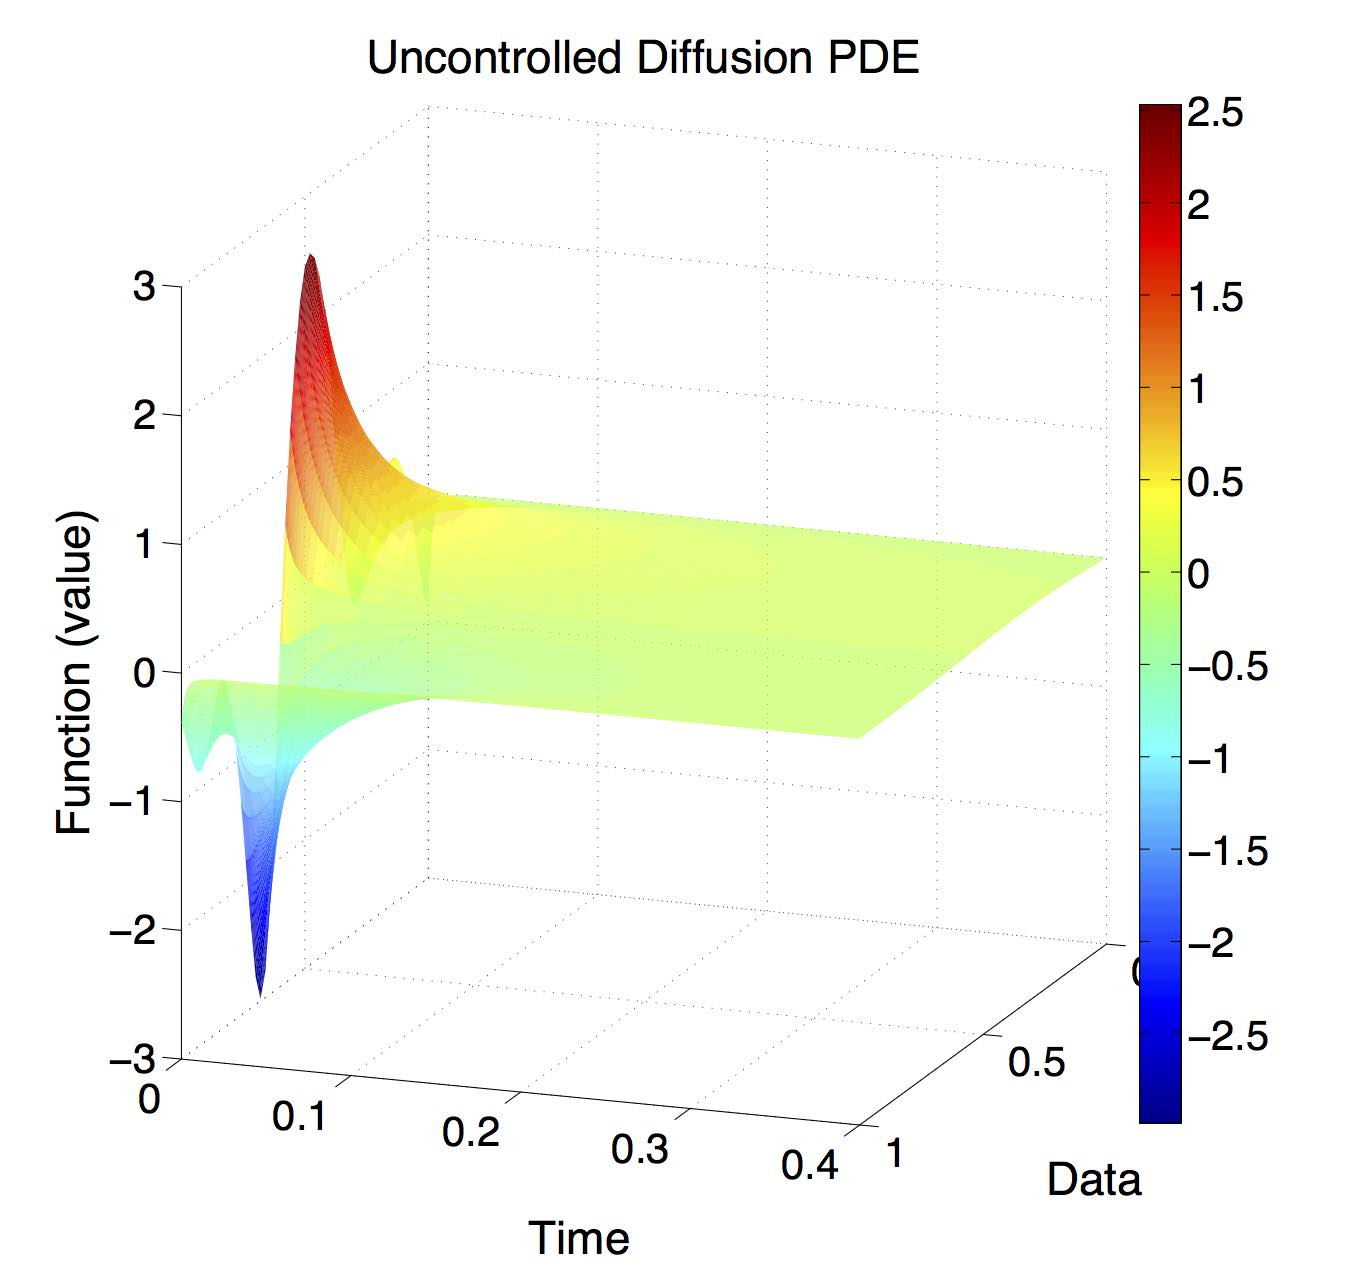
\includegraphics[width=0.45\columnwidth]{uncontrolled_pde_heat.jpg} 
%     \label{fig:uncontrolled_pde}}
% %     \subfloat[Initial function $f_{\text{init}}$ driven to $f_{\text{ref}}$ using kernel controller.]
% %     {
% %     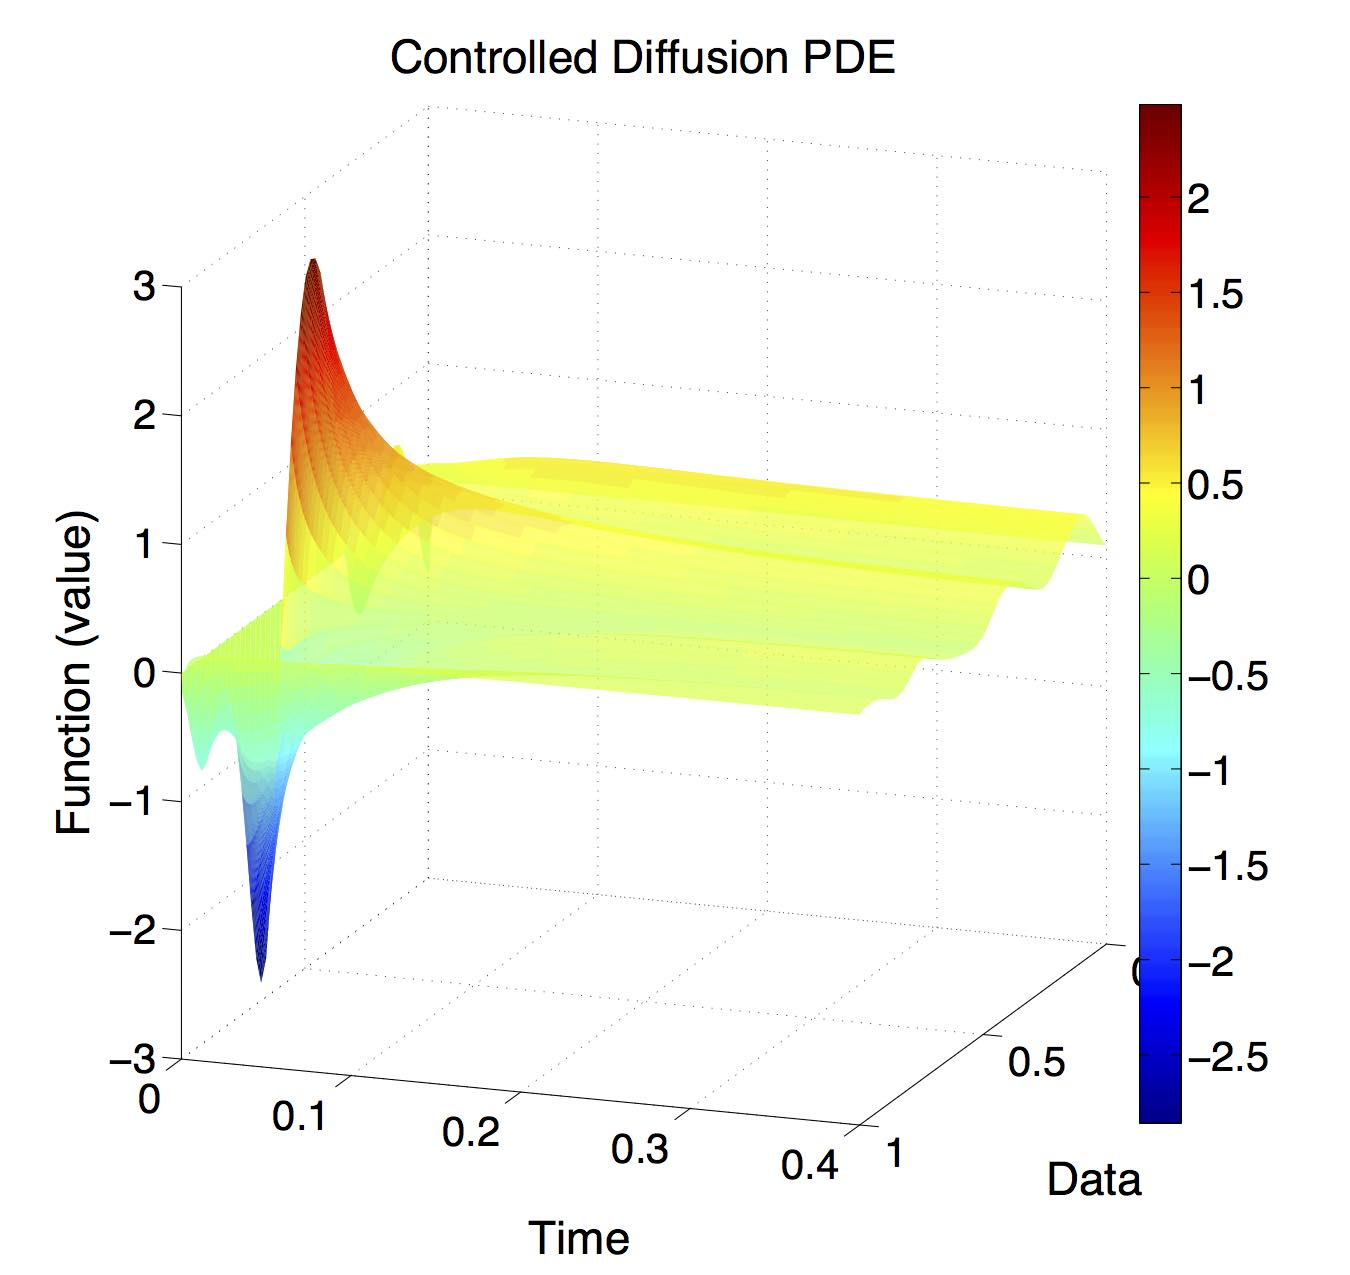
\includegraphics[width=0.5\columnwidth]{controlled_pde_heat.jpg} 
% %     \label{fig:controlled_pde}}    
% %     \\
%     \subfloat[Error in absolute value between controlled pde and $f_{\text{ref}}$. ]{
%     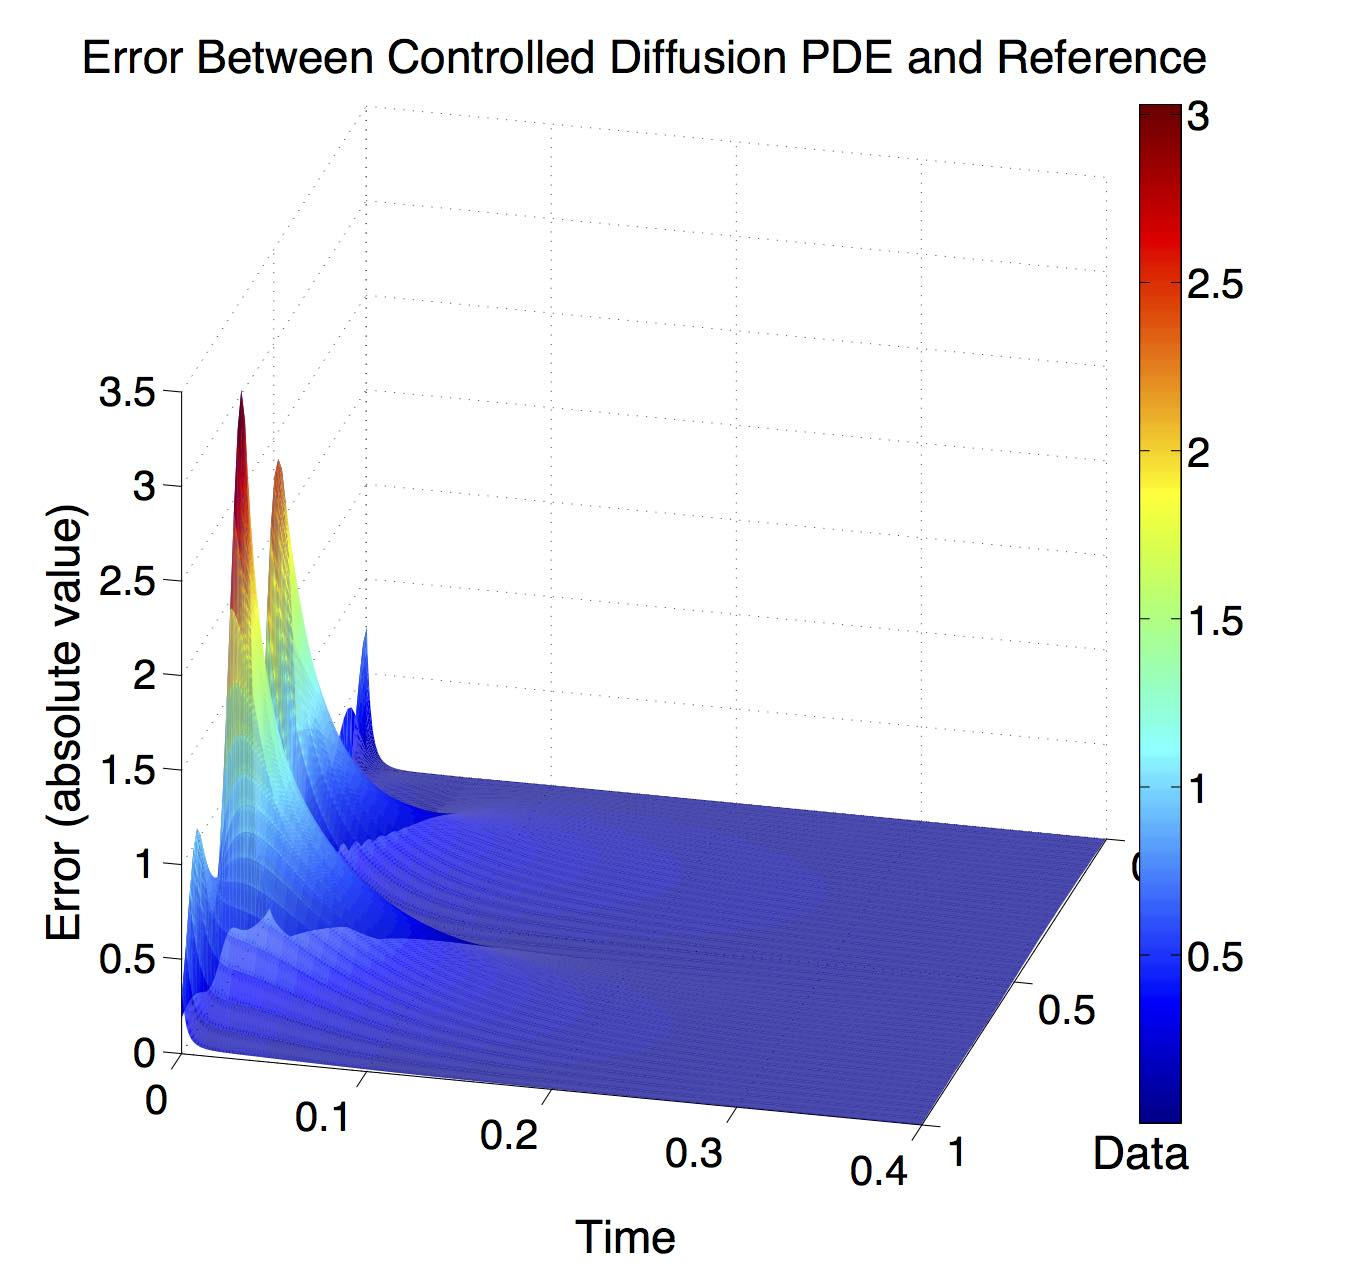
\includegraphics[width=0.45\columnwidth]{controlled_pde_error_heat.jpg} 
%     \label{fig:controlled_pde_error} }
%     \caption{Demonstration of the control of a linear diffusion equation.}     
% \end{figure}



\subsection{Comparison of Eigenvalues and Koopman modes with DMD}

In order to empirically verify our theoretical results, we compared the eigenvalues and Koopman modes derived from $\dualopApprox$ in our E-GP model with the eigenvalues and Koopman modes derived by the well-known Dynamic Mode Decomposition (DMD) algorithm using data from fluid flowing past a cylinder at different Reynolds numbers. The results are presented in figures \ref{fig:cfd_100_modes} and \ref{fig:eigenvalues}. As can be seen, the modes generated by E-GP match those generated by DMD at least as well as E-GP predictions match the original data.


\begin{figure*}[h]
	\centering
	\subfloat[0$^\circ$, real component]{
		\includegraphics[width=0.30\textwidth]{EGP/Re100/modeR_1a0deg}		}
	\subfloat[6$^\circ$, real component]{
		\includegraphics[width=0.30\textwidth]{EGP/Re100/modeR_1a6deg}		}
	\subfloat[12$^\circ$, real component]{
		\includegraphics[width=0.30\textwidth]{EGP/Re100/modeR_1a12deg}		}\\
	\subfloat[0$^\circ$, imaginary component]{
		\includegraphics[width=0.30\textwidth]{EGP/Re100/modeI_1a0deg}		}
	\subfloat[6$^\circ$, imaginary component]{
		\includegraphics[width=0.30\textwidth]{EGP/Re100/modeI_1a6deg}		}
	\subfloat[12$^\circ$, imaginary component]{
		\includegraphics[width=0.30\textwidth]{EGP/Re100/modeI_1a12deg}		}\\
	\subfloat[0$^\circ$, real component]{
		\includegraphics[width=0.30\textwidth]{DMD/Re100/modeR_1a0deg}		}
	\subfloat[6$^\circ$, real component]{
		\includegraphics[width=0.30\textwidth]{DMD/Re100/modeR_1a6deg}		}
	\subfloat[12$^\circ$, real component]{
		\includegraphics[width=0.30\textwidth]{DMD/Re100/modeR_1a12deg}		}\\
	\subfloat[0$^\circ$, imaginary component]{
		\includegraphics[width=0.30\textwidth]{DMD/Re100/modeI_1a0deg}		}
	\subfloat[6$^\circ$, imaginary component]{
		\includegraphics[width=0.30\textwidth]{DMD/Re100/modeI_1a6deg}		}
	\subfloat[12$^\circ$, imaginary component]{
		\includegraphics[width=0.30\textwidth]{DMD/Re100/modeI_1a12deg}		}
	\caption{Primary Koopman Modes, Re=100. (a-f) E-GP, (g-l) DMD}
	\label{fig:cfd_100_modes}
\end{figure*}

\begin{figure*}[h]
	\centering
	\subfloat[Re=100]{
		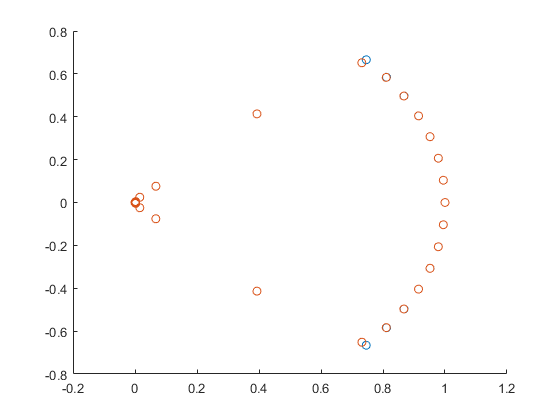
\includegraphics[width=0.48\textwidth]{eigenvalues/dmd100valscomp}		}
	\subfloat[Re=300]{
		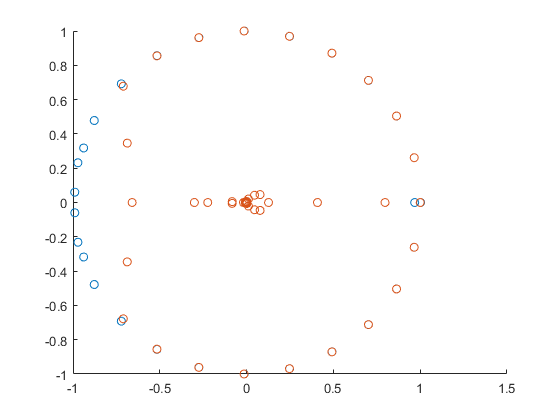
\includegraphics[width=0.48\textwidth]{eigenvalues/dmd300valscomp}		}\\
	\subfloat[Re=600]{
		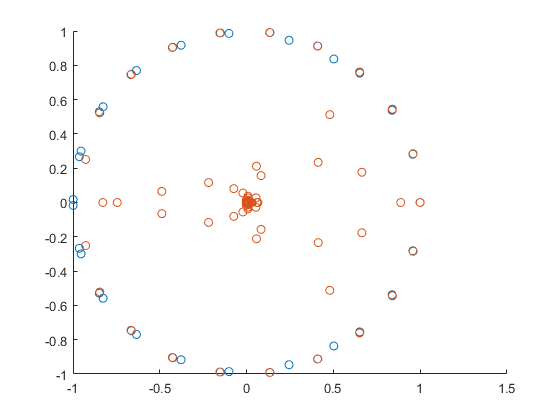
\includegraphics[width=0.48\textwidth]{eigenvalues/dmd600valscomp}		}
	\subfloat[Re=800]{
		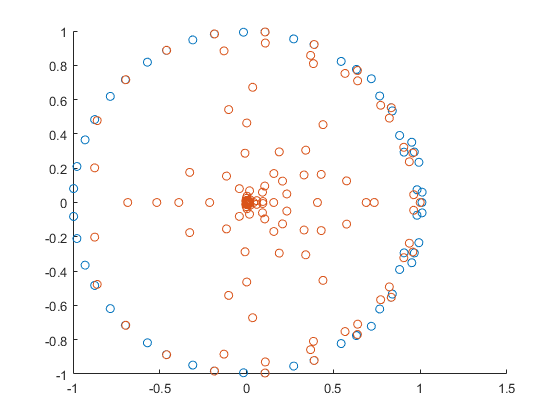
\includegraphics[width=0.48\textwidth]{eigenvalues/dmd800valscomp}		}\\
	\subfloat[Re=1000]{
		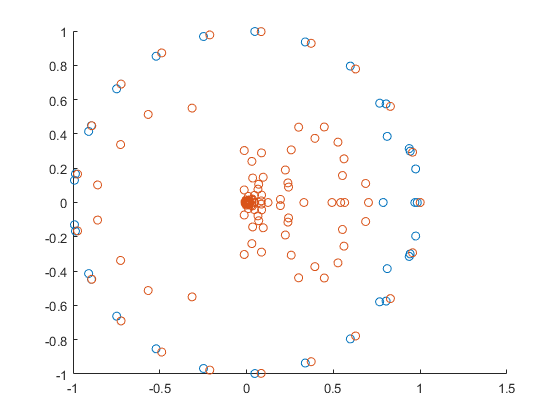
\includegraphics[width=0.48\textwidth]{eigenvalues/dmd1000valscomp}		}
	\caption{Eigenvalue Comparison}
	\label{fig:eigenvalues}
\end{figure*}


%\rr{
%\subsection{Paths for Moving Agents}
%To begin our investigation into the problem of finding best paths for sensing agents in motion, we constructed a number of simple synthetic spatiotemporally evolving systems for the agents to explore. One of these is displayed below \ref{fig:synthetic}. This is a system with two invariant subspaces, in each of which, two hills oscillate up and down in sync at a different frequency than the other invariant subspace. This is ideal for testing our methods. If successful, our methods should be able to (1) divide the space evenly between the two invariant subspaces, (2) be able to evaluate the spatial extent of the subspaces as roughly equivalent, (3) be able to identify the centers of each of the four hills as valuable waypoints, and (4) choose paths that travel between each of the hills equitably. In the example below, we used 100 centers with an RBF kernel with a bandwidth of 0.2 to train our E-GP model, though in testing we could also go as low as 20 centers.}
%
%
%\begin{figure*}[h]
%	\centering
%	\subfloat[Synthetic system with 2 invariant subspaces]{
%		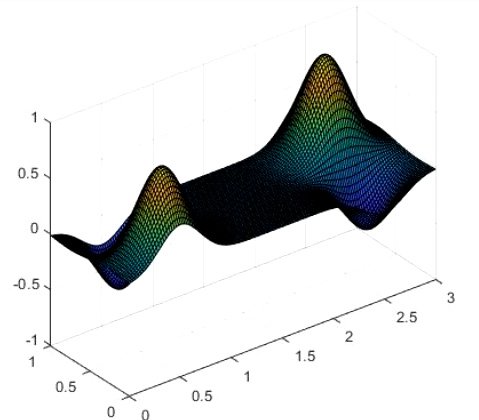
\includegraphics[width=0.30\textwidth]{synthetic23}
%		\label{fig:synthetic}	}
%	\subfloat[\small{Initial clustering of centers}]{
%		\includegraphics[width=0.30\textwidth]{init_cluster}
%		\label{fig:init_cluster}		}
%	\subfloat[\small{Final clustering of centers}]{
%		\includegraphics[width=0.34\textwidth]{final_cluster}
%		\label{fig:final_cluster}	}
%	\caption{Synthetic System Invariant Subspaces}
%\end{figure*}
%
%\rr{The $k$-means algorithm divides the system nicely through the middle, as expected.}
%
%\begin{figure*}[h]
%	\centering
%	\subfloat[Best Path Chosen for Synthetica Data Set]{
%		\includegraphics[width=0.30\textwidth]{pathS}
%		\label{fig:pathS}	}
%	\subfloat[\small{Convergence of State Prediction for Synthetic}]{
%		\includegraphics[width=0.30\textwidth]{convS}
%		\label{fig:convS}		}
%	\subfloat[\small{Best Path Chosen for CFD}]{
%		\includegraphics[width=0.34\textwidth]{path}
%		\label{fig:path}	}
%	\caption{More Results}
%\end{figure*}
%
%\rr{We found that the naive method of generating paths purely at random was largely futile, due to the large plain of zero values in-between the two invariant subspaces, which offer little in the way of meaningful data to correct the state estimate. By working with these synthetic data sets, we were able to test the three algorithms described in the previous section and demonstrate that they achieved the four criteria we laid out for them.}
%
%\rr{
%\subsubsection{Fluid Flow Past a Cylinder}
%
%To test our methods on challenging, realistic data sets, we used CFD methods to generate the states for a canonical fluid mechanics problem: flow past a cylinder at various Reynolds numbers, namely Re = 100, 300, 600, 800 and 1000. This deterministic, high-dimensional spatiotemporal dynamical system is well-studied in the fluid dynamics literature, both experimentally and numerically \cite{roshko1954cylinder, braza1986cylinder, rajani1986cylinder}. In our CFD simulation, we used a 4th-order polynomial expansion with spectral element method on the incompressible Navier-Stokes equation to generate the cylinder flow data. The spatial domain is $\left[-2,10\right]\times\left[-3,3\right]$, excluding the diameter-1 cylinder at the origin.  Neumann boundary conditions are applied to the far-field of the cylinder in the y-direction and the outlet of the flow field; and a Dirichlet boundary condition is applied to the inlet. The flow is unstable, periodic, and clearly nonlinear.
%
%For training the E-GP we used 600 centers with an RBF kernel with a bandwidth of 0.4. This output a $600\times600$ matrix $\dualopApprox$ which accurately captures the dynamics of the whole system. (Note that this reduces the size of the model by almost two orders of magnitude from the original CFD data).
%
%Since the CFD set has dynamics almost everywhere, most paths are able to converge to the state eventually, as long as they avoid wandering at the edges where the fluid velocity is semi-constant. However, we were able to demonstrate (as shown in the figures below) that our method of generating paths from valuable waypoints performs statistically much better than either purely random paths or random paths selected by the scoring algorithm.}%However, it is notable that a pre-designed lawnmower path failed to do as well as most random paths. Once again, the random paths generated and chosen by our methods did the best.
%
%\begin{figure*}[h]
%	\centering
%	\subfloat[\small{CFD system, Re=1000}]{
%		\includegraphics[width=0.30\textwidth]{snap1000_0}
%		\label{fig:cfd1000}	}
%	\subfloat[\small{Initial clustering of centers}]{
%		\includegraphics[width=0.30\textwidth]{init_clusterCFD}
%		\label{fig:cfd_init_cluster}		}
%	\subfloat[\small{Final clustering of centers}]{
%		\includegraphics[width=0.34\textwidth]{final_clusterCFD}
%		\label{fig:cfd_final_cluster}	}
%	\caption{CFD System Invariant Subspaces}
%\end{figure*}
%
%\begin{figure*}[h]
%	\centering
%	\subfloat[\small{Convergence of purely random paths}]{
%		\includegraphics[width=0.30\textwidth]{observer_worst}
%		\label{fig:observer_worst}	}
%	\subfloat[\small{Convergence of best scoring paths selected from random set}]{
%		\includegraphics[width=0.30\textwidth]{observer_middle}
%		\label{fig:observer_middle}		}
%	\subfloat[\small{Convergence of Best Scoring Path using Waypoints}]{
%		\includegraphics[width=0.34\textwidth]{observer_best}
%		\label{fig:observer_best}	}
%	\caption{Convergence results for CFD, showing mean, 15th, and 85th percentile path performance}
%\end{figure*}
